% Processed from chunks/10_dunham_euclid.md
% Repaired bilingual LaTeX fragment. Image paths are preserved from the source Markdown.

\section*{Dunham on Greek Geometry and Euclid / 邓纳姆论希腊几何与欧几里得}

\noindent\textbf{English.} Yet Euclid included no postulate to justify transferring lengths in this fashion. Where we expect an axiomatic dispensation allowing this procedure, we find nothing. Although his compass could draw a circle, he did not explicitly permit it to be locked into position and moved about. Euclid's is thus somewhat facetiously called a ``collapsible compass,'' a device that falls shut the instant it is lifted from the page.

\noindent\textbf{中文。} 然而，欧几里得并没有列入任何公设来说明可以用这种方式转移长度。我们本以为会看到一条公理化的许可，允许这种作图操作，可是在文本中却找不到。虽然他的圆规能够画圆，他并没有明说圆规可以固定开口后被移到别处。因此，人们多少带着玩笑意味地把欧几里得的圆规称为``可塌合圆规''：这种工具一离开纸面就会立刻合拢。

\begin{figure}[htbp]
\centering
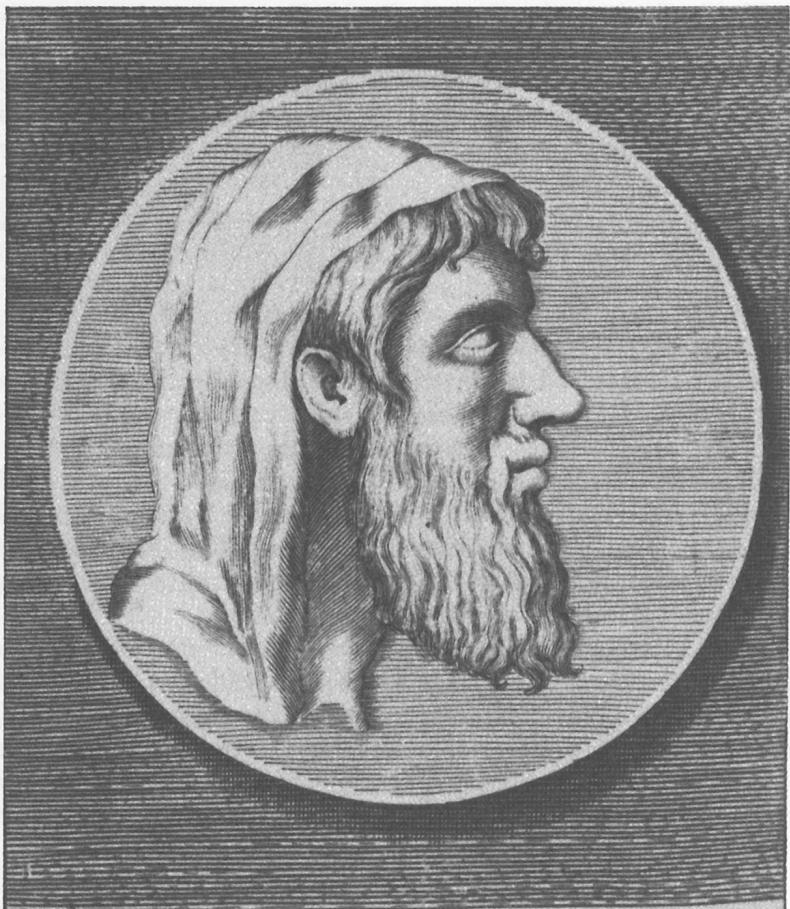
\includegraphics[width=0.42\linewidth]{images/7eaf4a037eb4c823f9b908dbe1242bbb0c9ea9ef550ceb0c57f8993e27459236.jpg}
\caption{Euclid portrait / 欧几里得肖像}
\end{figure}

\noindent\textbf{English.} The portrait caption identifies Euclid as the mathematician of Alexandria who taught under Ptolemy Lagus, and notes that his books of the \textit{Elements} were the most celebrated among works connected with music and geometry. The caption also says that the last two books were attributed to Hypsicles of Alexandria rather than to Euclid.

\noindent\textbf{中文。} 肖像题注称，欧几里得是亚历山大里亚的数学家，曾在托勒密·拉古斯统治时期任教；在与音乐和几何有关的著作中，他的《几何原本》最受赞誉。题注还说，最后两卷被归于亚历山大里亚的许普西克勒斯，而不是欧几里得本人。

\noindent\textbf{English.} This raises a serious question of logic: Did the esteemed Greek geometer forget to include a ``transfer of lengths'' postulate? Do we have here a Euclidean blunder?

\noindent\textbf{中文。} 这就提出了一个严肃的逻辑问题：这位备受尊崇的希腊几何学家是不是忘了加入一条``长度转移''公设？这里难道有一个欧几里得式的失误吗？

\noindent\textbf{English.} Not at all. As we shall see in a moment, Euclid had his reasons, reasons logically sound and very Greek in nature, for not including such a postulate. Rather than a blunder, this omission is evidence of his geometric acumen and organizational ability.

\noindent\textbf{中文。} 完全不是。我们马上会看到，欧几里得不加入这条公设自有其理由；这些理由在逻辑上站得住脚，也非常具有希腊数学的气质。与其说这是疏漏，不如说这一省略体现了他的几何洞察力和组织能力。

\noindent\textbf{English.} With postulates in place, Euclid introduced a few ``common notions,'' self-evident statements of a more general and less geometric nature. For instance, here we accept without proof that ``things which are equal to the same thing are also equal to one another,'' that ``if equals be added to equals, the wholes are equal,'' and that ``the whole is greater than the part.'' These are statements with which few will quibble.

\noindent\textbf{中文。} 在列出公设之后，欧几里得又引入若干``共同概念''，也就是一些更一般、几何色彩较少的不证自明的陈述。例如，我们在这里无需证明便承认：``等于同一事物的事物彼此相等''，``等量加等量，其和相等''，以及``整体大于部分''。这些说法很少会有人争辩。

\noindent\textbf{English.} Then he was ready to plunge in. With a huge body of geometry to deduce from a tiny collection of definitions, postulates, and common notions, where does one start? This is the sort of initial challenge known to freeze mathematicians and authors in their tracks. But if, as the Chinese tell us, a journey of a thousand miles begins with a single step, then Euclid's journey through geometry began with an equilateral triangle. The very first proposition of the \textit{Elements} was the construction, upon a given line segment, of just such a figure.

\noindent\textbf{中文。} 于是他便准备正式开始。要从少量定义、公设和共同概念出发，推出庞大的几何体系，究竟该从哪里下手？这种开端问题足以让数学家和作者都停在原地。但如果像中国谚语所说，千里之行始于足下，那么欧几里得的几何之旅便始于一个等边三角形。《几何原本》的第一条命题，正是在给定线段上作出这样一个图形。

\begin{figure}[htbp]
\centering
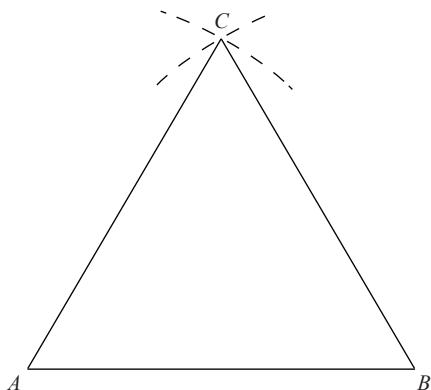
\includegraphics[width=0.32\linewidth]{images/84f5db85c3b186e63463411260378b177a27bfe2d50cb11f9cecead81e35076b.jpg}
\caption{Figure G.1 / 图 G.1}
\end{figure}

\noindent\textbf{English.} The argument is easy. Starting with given segment $AB$ in Figure G.1, we construct a circle with center at $A$ and radius $AB$ as permitted by postulate 3. Next, with center $B$ and radius $AB$, we invoke the same postulate to construct a second circle.

\noindent\textbf{中文。} 论证很简单。从图 G.1 中给定的线段 $AB$ 出发，按照公设 3，以 $A$ 为圆心、$AB$ 为半径作圆。接着仍用同一公设，以 $B$ 为圆心、$AB$ 为半径作第二个圆。

\noindent\textbf{English.} Let $C$ be the point where the circular arcs intersect. We then draw lines $AC$ and $BC$ by postulate 1, forming $\Delta ABC$. In this triangle, $AB$ and $AC$ are the same length because they are radii of the first circle; and $AB$ and $BC$ are the same length since they are radii of the second. Because things equal to the same thing are equal to each other, all three sides are mutually equal. By Euclid's definition, the triangle is equilateral and the proof is complete.

\noindent\textbf{中文。} 令 $C$ 为两段圆弧的交点。再由公设 1 连接 $AC$ 和 $BC$，得到 $\Delta ABC$。在这个三角形中，$AB$ 与 $AC$ 等长，因为它们同为第一个圆的半径；$AB$ 与 $BC$ 也等长，因为它们同为第二个圆的半径。由于等于同一事物的事物彼此相等，三条边便两两相等。按照欧几里得的定义，这个三角形是等边三角形，证明完成。

\noindent\textbf{English.} It is critical to observe that in using the compass for this construction, Euclid never needed to move it rigidly. After each arc was drawn, the compass can fall to pieces without affecting the proof in the least.

\noindent\textbf{中文。} 关键在于注意：在这个作图中，欧几里得从不需要把圆规保持开口不变地搬动。每画完一道圆弧，圆规即便散开，也丝毫不会影响证明。

\noindent\textbf{English.} But in the next two propositions of Book I, Euclid showed how a length could be transferred even with a compass that collapses. This means that length transfer was implied by the postulates already on the table. A new postulate to this end would have been unnecessary baggage, and Euclid was sharp enough to realize this.

\noindent\textbf{中文。} 但在第一卷随后的两个命题中，欧几里得说明了即使用可塌合圆规，也可以转移长度。这意味着``长度转移''其实已经由现有公设蕴含出来。为此另加一条公设只会成为多余的负担，而欧几里得敏锐地看出了这一点。

\begin{figure}[htbp]
\centering
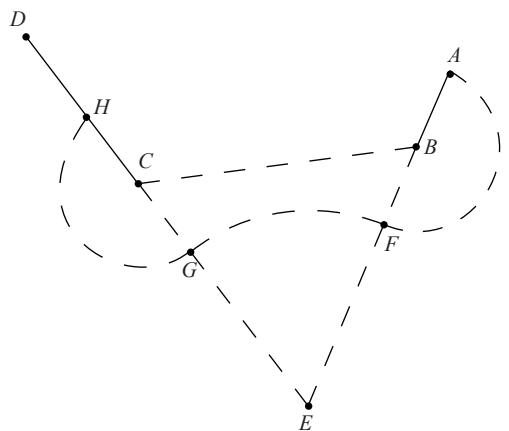
\includegraphics[width=0.44\linewidth]{images/fa5ce8f9fb874791de9f1c517fc1d12dd85942158f0f12f8aae1e298b3723d0a.jpg}
\caption{Figure G.2 / 图 G.2}
\end{figure}

\noindent\textbf{English.} His proofs, here combined into a single argument, were quite elegant. Suppose we have segment $AB$ as shown in Figure G.2 and wish to transfer its length onto the segment $CD$ emanating from the point $C$. First, use the straightedge and apply postulate 1 to draw the segment connecting $B$ and $C$. Then upon segment $BC$ construct equilateral triangle $BCE$; the legitimacy of this construction, of course, is exactly what was established in the previous proposition.

\noindent\textbf{中文。} 他的证明相当优雅；这里把两个证明合并成一个论证。假设我们有图 G.2 所示的线段 $AB$，并希望把它的长度转移到从点 $C$ 引出的线段 $CD$ 上。先用直尺并根据公设 1 作出连接 $B$ 与 $C$ 的线段。然后在线段 $BC$ 上作等边三角形 $BCE$；当然，这种作图的合法性正是上一命题已经建立的。

\noindent\textbf{English.} We then engage in a round of circle drawing. With center $B$ and radius $AB$, construct a circle meeting $BE$ at $F$; after the compass is picked up, suppose it collapses. With center $E$ and radius $EF$, draw a circle meeting $CE$ at $G$; again, the compass may collapse as we lift it from the page. With center $C$ and radius $CG$, draw a final circle meeting $CD$ at $H$. All of these constructions are permitted by Euclid's third postulate; none require a rigid compass.

\noindent\textbf{中文。} 接下来进行一连串画圆。以 $B$ 为圆心、$AB$ 为半径作圆，交 $BE$ 于 $F$；拿起圆规后，假定它塌合也无妨。再以 $E$ 为圆心、$EF$ 为半径作圆，交 $CE$ 于 $G$；离开纸面时圆规仍可塌合。最后以 $C$ 为圆心、$CG$ 为半径作圆，交 $CD$ 于 $H$。所有这些作图都由欧几里得的第三公设允许，没有一个需要刚性圆规。

\noindent\textbf{English.} Now we merely generate a string of equalities. For ease of notation, denote the length of segment $XY$ by $\overline{XY}$:
\[
\begin{array}{rl}
\overline{AB} &= \overline{BF} \quad \text{because they are radii of the same circle}\\
&= \overline{BE}-\overline{EF}\\
&= \overline{BE}-\overline{EG} \quad \text{because } EF \text{ and } EG \text{ are radii of the same circle}\\
&= \overline{CE}-\overline{EG} \quad \text{because the three sides of } \Delta BCE \text{ are equally long}\\
&= \overline{CG}\\
&= \overline{CH} \quad \text{because again we have radii of the same circle.}
\end{array}
\]

\noindent\textbf{中文。} 现在只需列出一串等式。为记号方便，用 $\overline{XY}$ 表示线段 $XY$ 的长度：
\[
\begin{array}{rl}
\overline{AB} &= \overline{BF} \quad \text{因为它们是同一圆的半径}\\
&= \overline{BE}-\overline{EF}\\
&= \overline{BE}-\overline{EG} \quad \text{因为 } EF \text{ 与 } EG \text{ 是同一圆的半径}\\
&= \overline{CE}-\overline{EG} \quad \text{因为 } \Delta BCE \text{ 的三边等长}\\
&= \overline{CG}\\
&= \overline{CH} \quad \text{因为这里又是同一圆的半径。}
\end{array}
\]

\noindent\textbf{English.} The beginning and end of this chain reveal that $\overline{AB}=\overline{CH}$. Therefore the initial length of $AB$ has been transferred onto segment $CD$ as required, yet nowhere did we have to pick up a compass and move it rigidly.

\noindent\textbf{中文。} 这条等式链的开头和结尾表明 $\overline{AB}=\overline{CH}$。因此，原来 $AB$ 的长度已经按要求转移到了线段 $CD$ 上，而在整个过程中，我们从未需要拿起圆规并保持开口不变地移动它。

\noindent\textbf{English.} The surprising conclusion of this proof is that constructions seeming to require a noncollapsing compass can actually be accomplished with a collapsible one. As he subsequently developed his geometry, Euclid could therefore legitimately transfer a length from one place to another as if with a rigid compass, his rationale being the just-proved theorem. By getting it out of the way so early, and so simply, he was free to use it in all that followed.

\noindent\textbf{中文。} 这个证明令人惊讶的结论是：那些看起来需要不塌合圆规的作图，实际上可以用可塌合圆规完成。因此，在随后发展几何时，欧几里得可以正当地像使用刚性圆规那样把长度从一处转到另一处，其依据正是刚刚证明的定理。他如此早、如此简洁地处理掉这一点，便能在后续所有论证中自由使用它。

\noindent\textbf{English.} At this point some readers may be stifling a yawn, regarding the whole business as much ado about nothing. After all, everyone knows that stationery stores sell cheap metal compasses that are made to stay open, and surely it would have done no great damage for Euclid to have included an extra postulate to that effect.

\noindent\textbf{中文。} 读到这里，有些读者也许已经强忍哈欠，觉得整件事不过是小题大做。毕竟人人都知道，文具店出售的廉价金属圆规本来就能保持开口；欧几里得即便为此多添一条公设，似乎也不会造成多大损害。

\noindent\textbf{English.} Adherents of this position, we believe, have not yet gotten into the spirit of formal Greek geometry. First, the real-world existence of rigid compasses has no bearing on the development of ideal concepts. Second, stationery stores had not yet been invented. Third, and most crucially, Euclid would not have wanted to add an unnecessary postulate to his list. Why assume something that could be derived from other assumptions? It would make his postulates less pure, less streamlined, and less perfect, thereby violating an aesthetic principle rather than a mathematical one.

\noindent\textbf{中文。} 我们认为，持这种看法的人还没有进入希腊形式几何的精神。第一，现实世界中是否存在刚性圆规，与理想概念的发展无关。第二，当时还没有文具店。第三，也是最关键的一点，欧几里得不会愿意在自己的清单中加入不必要的公设。既然某件事可以由其他假设推出，为什么还要把它当作假设？那会使他的公设不够纯粹、不够简洁、不够完美；它违反的不是数学原则，而是审美原则。

\noindent\textbf{English.} That aesthetic considerations were critical for the Greek mathematician is obvious. In Euclid's proof above we glimpse what Ivor Thomas meant when he wrote:

\begin{quote}
\noindent\textbf{English.} A feature which cannot fail to impress a modern mathematician is the perfection of form in the work of the great Greek geometers. This perfection of form, which is another expression of the same genius that gave us the Parthenon and the plays of Sophocles, is found equally in the proof of individual propositions and in the ordering of those separate propositions into books; it reaches its height, perhaps, in the \textit{Elements} of Euclid.

\noindent\textbf{中文。} 现代数学家必定会深受触动的一个特征，是伟大希腊几何学家作品中形式的完美。这种形式的完美，是创造出帕特农神庙和索福克勒斯戏剧的同一天才的另一种表现；它既见于单个命题的证明，也见于把各个命题编排成卷册的秩序之中；也许，它在欧几里得的《几何原本》中达到了顶峰。
\end{quote}

\noindent\textbf{English.} We now move deeper into Book I to see further evidence of Euclid's genius. After disposing of the collapsible compass in propositions 2 and 3, Euclid proved the so-called side-angle-side, or SAS, congruence scheme in proposition 4. That is, if we have triangles $ABC$ and $DEF$ in which $\overline{AB}=\overline{DE}$, $\overline{AC}=\overline{DF}$, and the included angles $\alpha=\delta$, then the triangles are congruent, meaning they have precisely the same size and shape. In other words, if $\Delta DEF$ were picked up and placed atop $\Delta ABC$, the two would coincide perfectly, line for line, angle for angle, point for point.

\noindent\textbf{中文。} 现在我们深入第一卷，看看欧几里得天才的更多证据。在命题 2 和命题 3 中处理完``可塌合圆规''之后，欧几里得在命题 4 中证明了所谓的边角边，即 SAS 全等判定。也就是说，若有三角形 $ABC$ 和 $DEF$，其中 $\overline{AB}=\overline{DE}$，$\overline{AC}=\overline{DF}$，且夹角 $\alpha=\delta$，那么这两个三角形全等，意思是它们有完全相同的大小和形状。换言之，如果把 $\Delta DEF$ 拿起来放在 $\Delta ABC$ 上，两者会线对线、角对角、点对点地完全重合。

\begin{figure}[htbp]
\centering
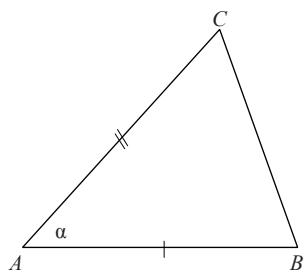
\includegraphics[width=0.28\linewidth]{images/3e123e38e33ce41d4eced941a453c9d23cc1fb1f3823f6bee06e8fcfcf595e74.jpg}\quad
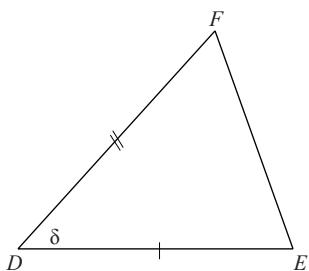
\includegraphics[width=0.28\linewidth]{images/2bd811776486f854a6498e3c7308b4cd40dca32e62e6d03eaf1aef000381d89b.jpg}
\caption{Figure G.3 / 图 G.3}
\end{figure}

\noindent\textbf{English.} In Euclid's hands, triangle congruence was the key to proving geometric propositions. Later he established the additional congruence patterns of side-side-side (SSS) in proposition 8, and angle-side-angle (ASA) and angle-angle-side (AAS) in proposition 26.

\noindent\textbf{中文。} 在欧几里得手中，三角形全等是证明几何命题的关键。后来他又在命题 8 中建立了边边边（SSS）全等判定，并在命题 26 中建立了角边角（ASA）和角角边（AAS）全等判定。

\noindent\textbf{English.} Proposition 5 of Book I proved that the base angles of an isosceles triangle are congruent. As noted, this result has been attributed to Thales, but the proof in the \textit{Elements} is probably Euclid's own. Although we shall not give it here, we note that it was accompanied by the diagram in Figure G.4. This configuration, which suggests a bridge to vivid imaginations, may account for calling proposition 5 the \textit{pons asinorum}, or bridge of asses. According to tradition, dullards, that is, asses, find the proof beyond them and thus cannot cross this logical bridge into the geometric promised land of the \textit{Elements}.

\noindent\textbf{中文。} 第一卷命题 5 证明了等腰三角形的底角全等。如前所述，这一结果曾被归于泰勒斯，但《几何原本》中的证明很可能是欧几里得自己的。虽然我们这里不列出该证明，但要注意它配有图 G.4。这个图形在想象力丰富的人看来像一座桥，这也许解释了为什么命题 5 被称为 \textit{pons asinorum}，即``愚驴之桥''。按照传统，迟钝的人，也就是所谓的``驴''，理解不了这个证明，因此无法跨过这座逻辑之桥，进入《几何原本》的几何应许之地。

\begin{figure}[htbp]
\centering
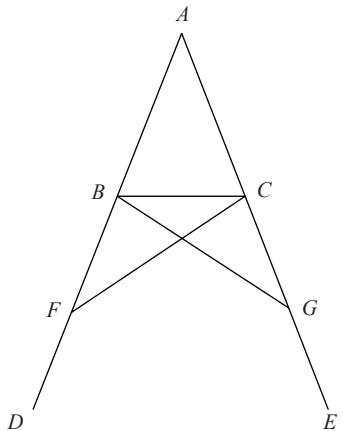
\includegraphics[width=0.42\linewidth]{images/67343c2087e15ce1a36ae4fa638c9ba61463f662a18f6217e0c85e2596f8f2a3.jpg}
\caption{Figure G.4 / 图 G.4}
\end{figure}

\noindent\textbf{English.} If weak students were likened to asses, Euclid himself met a similar fate at the hands of the Epicureans for his proof of proposition 20. To see why, we must describe a few of the intervening theorems of Book I.

\noindent\textbf{中文。} 如果薄弱的学生会被比作驴，那么欧几里得本人也因为命题 20 的证明，在伊壁鸠鲁学派那里遭遇了类似的命运。要看清原因，我们必须先说明第一卷中间的几个定理。

\noindent\textbf{English.} After crossing the \textit{pons asinorum}, Euclid showed how to bisect angles and construct perpendiculars with compass and straightedge and soon arrived at one of the critical theorems of Book I, commonly known as the exterior angle theorem. This result, which appeared as proposition 16, guaranteed that the exterior angle of any triangle exceeds either of the opposite and interior angles. That is, if we begin with $\Delta ABC$ and extend side $BC$ rightward to $D$, then both $\alpha$ and $\beta$ are less than $\angle ACD$.

\noindent\textbf{中文。} 跨过``愚驴之桥''后，欧几里得说明了如何用圆规和直尺作角平分线、作垂线，并很快到达第一卷的一个关键定理，通常称为外角定理。这个出现在命题 16 中的结果保证，任意三角形的外角都大于任一不相邻内角。也就是说，如果从 $\Delta ABC$ 出发，把边 $BC$ 向右延长到 $D$，那么 $\alpha$ 和 $\beta$ 都小于 $\angle ACD$。

\begin{figure}[htbp]
\centering
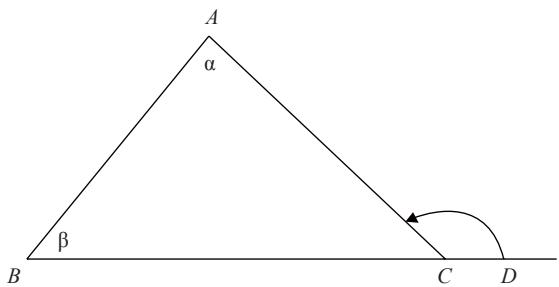
\includegraphics[width=0.42\linewidth]{images/9fe2f5e7a9593709c5c05a4446fb2f56e135c53e3ccd705c3040aeeb0e47476b.jpg}
\caption{Figure G.5 / 图 G.5}
\end{figure}

\noindent\textbf{English.} The exterior angle theorem was the first geometric inequality in the \textit{Elements}. Where Euclid had previously shown sides or angles to be equal, as in the \textit{pons asinorum}, he here proved certain angles to be unequal. This theorem would play a significant role in the remainder of Book I.

\noindent\textbf{中文。} 外角定理是《几何原本》中的第一个几何不等式。此前欧几里得证明的是边或角相等，例如``愚驴之桥''；而在这里，他证明某些角不相等。这个定理将在第一卷余下部分发挥重要作用。

\noindent\textbf{English.} This brings us to another inequality, proposition 19, whose diagram appears in Figure G.6. Euclid stated it as, ``In any triangle the greater angle is subtended by the greater side,'' which in more modern notation becomes:

\noindent\textbf{中文。} 这把我们带到另一个不等式，即命题 19，其图形见图 G.6。欧几里得把它表述为：``在任意三角形中，较大的角由较大的边所对。'' 用较现代的记号写就是：

\noindent\textbf{English.} \textbf{Proposition 19.} In $\Delta ABC$, if $\beta>\alpha$, then $\overline{AC}>\overline{BC}$, that is, $b>a$.

\noindent\textbf{中文。} \textbf{命题 19。} 在 $\Delta ABC$ 中，若 $\beta>\alpha$，则 $\overline{AC}>\overline{BC}$，也就是 $b>a$。

\noindent\textbf{English.} \textbf{Proof.} Here we assume that $\beta>\alpha$. It is our job to prove that side $AC$ opposite $\angle ABC$ is longer than side $BC$ opposite $\angle BAC$.

\noindent\textbf{中文。} \textbf{证明。} 这里假设 $\beta>\alpha$。我们的任务是证明，与 $\angle ABC$ 相对的边 $AC$ 长于与 $\angle BAC$ 相对的边 $BC$。

\noindent\textbf{English.} Euclid separately considered the three possible cases: $b=a$, $b<a$, and $b>a$. His strategy was to show that the first two are impossible and thereby conclude that the third case must hold, as the theorem asserted. Such a technique is called a double \textit{reductio ad absurdum}, or a proof by double contradiction. This powerful logical strategy was nowhere better employed than in Greek mathematics. Here is how Euclid handled it.

\noindent\textbf{中文。} 欧几里得分别考察了三种可能情形：$b=a$、$b<a$ 和 $b>a$。他的策略是说明前两种不可能，从而得出第三种必然成立，正如定理所断言。这种技巧称为双重归谬，或双重反证。没有哪个地方比希腊数学更善于运用这种强有力的逻辑策略。欧几里得的处理如下。

\noindent\textbf{English.} \textbf{Case 1.} Suppose $b=a$.

\noindent\textbf{中文。} \textbf{情形 1。} 假设 $b=a$。

\noindent\textbf{English.} Referring to Figure G.6, we have $\overline{BC}=a=b=\overline{AC}$. This makes $\Delta ABC$ isosceles and so, invoking the \textit{pons asinorum}, we conclude that the base angles are themselves congruent. That is, $\angle BAC=\angle ABC$, or equivalently $\alpha=\beta$. But this contradicts the initial assumption that $\beta>\alpha$. Hence we dismiss Case 1 as impossible.

\noindent\textbf{中文。} 参照图 G.6，我们有 $\overline{BC}=a=b=\overline{AC}$。于是 $\Delta ABC$ 是等腰三角形；调用``愚驴之桥''，可知其底角全等。也就是说，$\angle BAC=\angle ABC$，等价地，$\alpha=\beta$。但这与初始假设 $\beta>\alpha$ 矛盾。因此情形 1 不可能。

\begin{figure}[htbp]
\centering
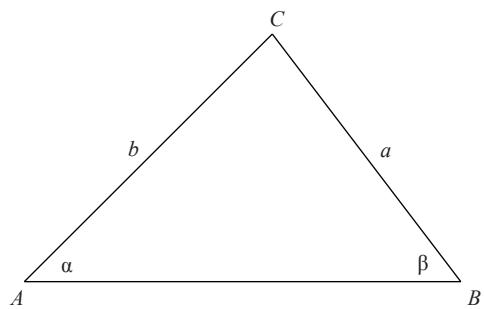
\includegraphics[width=0.42\linewidth]{images/f7e1b267dc666d8de877e4a633130d80b036cdacf94ddd4b5aea15c997f8992c.jpg}
\caption{Figure G.6 / 图 G.6}
\end{figure}

\noindent\textbf{English.} \textbf{Case 2.} Suppose $b<a$.

\noindent\textbf{中文。} \textbf{情形 2。} 假设 $b<a$。

\noindent\textbf{English.} Here we have the situation depicted in Figure G.7. Because $AC$ is assumed to be shorter than $BC$, we can construct segment $CD$ of length $b$ where $D$ falls within the longer side $BC$. Then draw $AD$ to form $\Delta ADC$. This triangle, having two sides of length $b$, is isosceles and therefore has congruent base angles $\angle DAC$ and $\angle ADC$. But applying the exterior angle theorem to the narrow $\Delta ABD$, we deduce that
\[
\begin{array}{rl}
\beta &= \text{interior } \angle ABD\\
&< \text{exterior } \angle ADC \quad \text{by the exterior angle theorem}\\
&= \angle DAC \quad \text{because } \Delta DAC \text{ is isosceles}\\
&< \angle BAC \quad \text{because the whole is greater than the part}\\
&= \alpha.
\end{array}
\]

\noindent\textbf{中文。} 这里的情形如图 G.7 所示。由于假设 $AC$ 短于 $BC$，我们可以在较长的边 $BC$ 内取一点 $D$，使线段 $CD$ 的长度为 $b$。再连接 $AD$，形成 $\Delta ADC$。这个三角形有两条边长为 $b$，因此是等腰三角形，从而底角 $\angle DAC$ 与 $\angle ADC$ 全等。把外角定理用于狭长的 $\Delta ABD$，得到
\[
\begin{array}{rl}
\beta &= \text{内角 } \angle ABD\\
&< \text{外角 } \angle ADC \quad \text{由外角定理}\\
&= \angle DAC \quad \text{因为 } \Delta DAC \text{ 是等腰三角形}\\
&< \angle BAC \quad \text{因为整体大于部分}\\
&= \alpha.
\end{array}
\]

\begin{figure}[htbp]
\centering
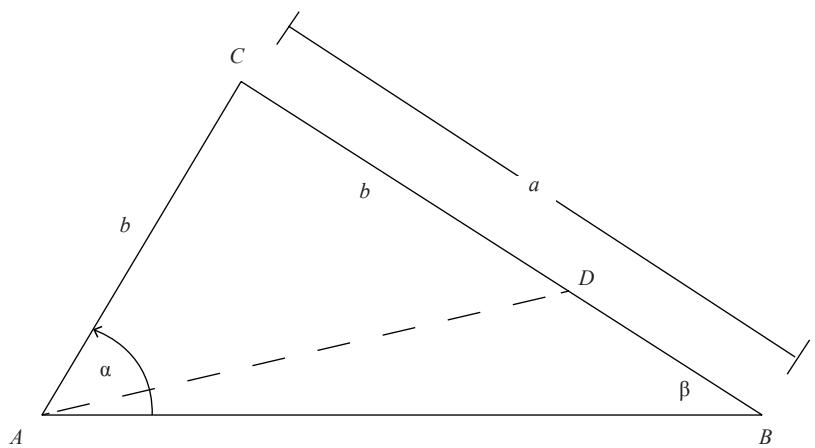
\includegraphics[width=0.42\linewidth]{images/886014fc2a084db7af8e4c02c433fe3726c033b2487e545890387c57e8b73565.jpg}
\caption{Figure G.7 / 图 G.7}
\end{figure}

\noindent\textbf{English.} In other words, $\beta<\alpha$, which contradicts the theorem's original stipulation that $\beta>\alpha$. Case 2, leading as it does to a contradiction, also bites the dust. We are left with:

\noindent\textbf{中文。} 换言之，$\beta<\alpha$，这与定理原先的规定 $\beta>\alpha$ 相矛盾。情形 2 既然导致矛盾，也被排除。剩下的只有：

\noindent\textbf{English.} \textbf{Case 3.} $b>a$.

\noindent\textbf{中文。} \textbf{情形 3。} $b>a$。

\noindent\textbf{English.} This must be true because no alternatives remain, and the theorem is proved.

\noindent\textbf{中文。} 因为已经没有其他可能，这一情形必定为真，定理得证。

\noindent\textbf{English.} We now have reached the proposition that so troubled the Epicurean philosophers. On the surface it sounds harmless enough:

\noindent\textbf{中文。} 现在我们到达了那个令伊壁鸠鲁派哲学家很不满的命题。表面上它听起来相当无害：

\noindent\textbf{English.} \textbf{Proposition 20.} In any triangle two sides taken together in any manner are greater than the remaining one.

\noindent\textbf{中文。} \textbf{命题 20。} 在任意三角形中，任取两边之和都大于余下的一边。

\noindent\textbf{English.} Why the controversy? Why the derision? We quote the commentator Proclus:

\noindent\textbf{中文。} 为什么会有争议？为什么会有嘲笑？我们引用评注家普罗克洛的话：

\begin{quote}
\noindent\textbf{English.} The Epicureans are wont to ridicule this theorem, saying it is evident even to an ass and needs no proof; it is as much the mark of an ignorant man, they say, to require persuasion of evident truths as to believe what is obscure without question. That the present theorem is known to an ass they make out from the observation that, if straw is placed at one extremity of the sides, an ass in quest of provender will make his way along the one side and not by way of the two others.

\noindent\textbf{中文。} 伊壁鸠鲁派惯于嘲笑这个定理，说它连驴都看得出来，根本不需要证明；他们说，对显然的真理还要求别人说服自己，正如对晦暗之物不加追问就相信一样，都是无知者的标志。他们说连驴都知道这个定理，是因为观察到：如果把草放在边的一端，寻找饲料的驴会沿着一条边走过去，而不会绕另外两条边过去。
\end{quote}

\noindent\textbf{English.} In short, even a dumb animal knows to take the straight route from $C$ to $B$ in Figure G.8 rather than go the long way around via $A$. So why, the Epicureans asked, did Euclid bother to prove something so blatantly obvious? Proclus gave an answer:

\noindent\textbf{中文。} 简言之，即便是不会说话的动物也知道，在图 G.8 中应走从 $C$ 到 $B$ 的直路，而不是经由 $A$ 绕远路。所以伊壁鸠鲁派问：欧几里得为什么要费心证明如此显而易见的事情？普罗克洛给出了回答：

\begin{quote}
\noindent\textbf{English.} It should be replied that, granting the theorem is evident to sense-perception, it is still not clear for scientific thought. Many things have this character; for example, that fire warms. This is clear to perception, but it is the task of science to find out how it warms.

\noindent\textbf{中文。} 应当回答说，即便承认这个定理对感官知觉是明显的，它对科学思想仍然并不清楚。许多事情都有这种性质；例如火会使人感到温暖。对知觉而言这是清楚的，但科学的任务是弄清它怎样使人温暖。
\end{quote}

\begin{figure}[htbp]
\centering
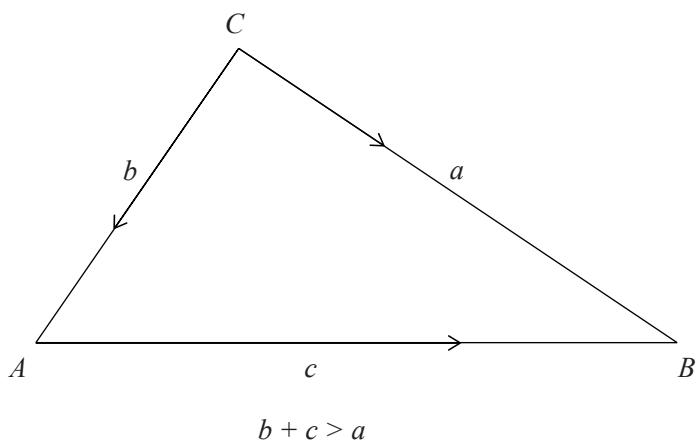
\includegraphics[width=0.42\linewidth]{images/e2cd42c9578b762ce58bcb4261733970990aaec7d5d6b3e0dc01b22a793f970f.jpg}
\caption{Figure G.8 / 图 G.8}
\end{figure}

\noindent\textbf{English.} In the Euclidean spirit, the spirit that so typified Greek geometry, we must employ our faculties of reason to demonstrate that which instinct already knows. Even a seemingly self-evident proposition cries out for a proof, and this Euclid was only too happy to provide. Building upon previous results, he reasoned as follows:

\noindent\textbf{中文。} 在欧几里得精神中，也就是希腊几何最典型的精神中，我们必须运用理性能力来证明本能已经知道的事情。即便一个看似不证自明的命题也呼唤证明，而欧几里得非常乐意提供这样的证明。基于先前结果，他这样论证：

\noindent\textbf{English.} \textbf{Proposition 20.} In $\Delta ABC$, $\overline{AC}+\overline{AB}>\overline{BC}$, that is, $b+c>a$.

\noindent\textbf{中文。} \textbf{命题 20。} 在 $\Delta ABC$ 中，$\overline{AC}+\overline{AB}>\overline{BC}$，也就是 $b+c>a$。

\noindent\textbf{English.} \textbf{Proof.} In Figure G.9, extend side $BA$ to $D$ so that $\overline{AD}=\overline{AC}=b$ and therefore $\overline{BD}=b+c$. This construction generates $\Delta DAC$, which is isosceles because it has two sides of length $b$. Considering the large $\Delta BDC$, we note that
\[
\begin{array}{rl}
\angle BCD &> \angle ACD \quad \text{because the whole is greater than the part}\\
&= \angle BDC \quad \text{because these are base angles of isosceles } \Delta DAC.
\end{array}
\]

\noindent\textbf{中文。} \textbf{证明。} 在图 G.9 中，把边 $BA$ 延长到 $D$，使 $\overline{AD}=\overline{AC}=b$，因而 $\overline{BD}=b+c$。这个作图生成 $\Delta DAC$，它有两条边长为 $b$，所以是等腰三角形。考察较大的 $\Delta BDC$，注意到
\[
\begin{array}{rl}
\angle BCD &> \angle ACD \quad \text{因为整体大于部分}\\
&= \angle BDC \quad \text{因为它们是等腰三角形 } \Delta DAC \text{ 的底角。}
\end{array}
\]

\noindent\textbf{English.} So $\angle BCD$ is greater than $\angle BDC$. As Euclid had just proved that the greater side is opposite the greater angle, it follows that $\overline{BD}>\overline{BC}$; in other words, $b+c>a$, which is exactly what was to be proved.

\noindent\textbf{中文。} 因此 $\angle BCD$ 大于 $\angle BDC$。由于欧几里得刚刚证明较大角对较大边，所以可得 $\overline{BD}>\overline{BC}$；换言之，$b+c>a$，这正是所要证明的。

\begin{figure}[htbp]
\centering
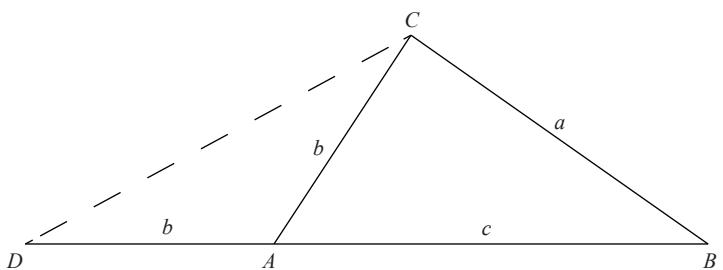
\includegraphics[width=0.42\linewidth]{images/37496d2ca430aa89754c56d324b80bae2c289097df3e5919bca7dbbcce3db9de.jpg}
\caption{Figure G.9 / 图 G.9}
\end{figure}

\noindent\textbf{English.} This is a splendid little proof. It has its subtleties, its clever use of inequalities, its quiet elegance.

\noindent\textbf{中文。} 这是一个精彩的小证明。它有细腻之处，有对不等式的巧妙运用，也有一种安静的优雅。

\noindent\textbf{English.} In Sir Arthur Conan Doyle's \textit{A Study in Scarlet}, Dr. Watson described the deductive powers of Sherlock Holmes in these words: ``His conclusions were as infallible as so many propositions of Euclid.'' Watson was not alone in his high opinion of the Greek geometer. Centuries ago, the Arabic scholar al-Qifti said of Euclid, ``nay, there was no one even of later date who did not walk in his footsteps,'' and the incomparable Albert Einstein added his own tribute: ``If Euclid failed to kindle your youthful enthusiasm, then you were not born to be a scientific thinker.''

\noindent\textbf{中文。} 在阿瑟·柯南·道尔爵士的《血字的研究》中，华生医生这样描述夏洛克·福尔摩斯的演绎能力：``他的结论像欧几里得的诸多命题一样无懈可击。'' 并非只有华生如此推崇这位希腊几何学家。数百年前，阿拉伯学者阿尔-基夫提评价欧几里得说：``甚至在后世，也没有一个人不是沿着他的足迹前行。'' 无与伦比的阿尔伯特·爱因斯坦也献上自己的赞词：``如果欧几里得未能点燃你少年时代的热情，那么你天生就不是科学思想者。''

\noindent\textbf{English.} What we have considered thus far, of course, is just the tip of the iceberg, just a sampler of what historian Morris Kline calls the Greeks' ``grand exercise in logic.'' We must leave them at this point. But in a sense, no mathematician can leave behind the legacy of the classical geometers. They gave demonstrative mathematics its start, honed its logical tools, and aimed it in directions it has traveled ever since. We end with the words of the twentieth-century British mathematician G. H. Hardy: ``The Greeks ... spoke a language which modern mathematicians can understand; as Littlewood said to me once, they are not clever schoolboys or scholarship candidates, but Fellows of another college.''

\noindent\textbf{中文。} 当然，我们迄今所考察的只是冰山一角，只是历史学家莫里斯·克莱因所谓希腊人``逻辑的宏大操练''的一个样本。我们必须在此暂别他们。但从某种意义上说，没有哪位数学家能够真正离开古典几何学家的遗产。他们开创了论证数学，磨砺了它的逻辑工具，并把它引向了此后一直行进的方向。我们以二十世纪英国数学家 G. H. 哈代的话作为结尾：``希腊人……说的是现代数学家能够理解的语言；正如利特尔伍德有一次对我说的，他们不是聪明的学生或奖学金候选人，而是另一所学院的研究员。''

\noindent\textbf{English.} There is no arguing with Hardy when he says, ``Greek mathematics is the real thing.''

\noindent\textbf{中文。} 哈代说``希腊数学是真正的数学''时，我们无法反驳。

\begin{center}

\includegraphics[width=0.26\linewidth]{images/abcb3bf131696c0acfd75ec97f91d1522860409ebbea163aaff717510f61489b.jpg}\quad
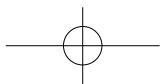
\includegraphics[width=0.26\linewidth]{images/948c10988b3b8098710740c00c6c465fbc59bcfc37867c9b395adc7af73e16aa.jpg}\quad

\includegraphics[width=0.26\linewidth]{images/abda016953b0c39c0618f44dccbcfdfda7411c9a08e2266903d730906f97cb2e.jpg}
\end{center}

\section*{Text 11b: \textit{Elements}, Book I / 文本 11b：《几何原本》第一卷}

\noindent\textbf{English.} From \textit{Elements} by Euclid.

\noindent\textbf{中文。} 选自欧几里得《几何原本》。

\subsection*{Definitions / 定义}

\begin{enumerate}
\item \textbf{English.} A point is that which has no part. \par\textbf{中文。} 点是没有部分的东西。
\item \textbf{English.} A line is breadthless length. \par\textbf{中文。} 线是无宽之长。
\item \textbf{English.} The extremities of a line are points. \par\textbf{中文。} 线的端是点。
\item \textbf{English.} A straight line is a line which lies evenly with the points on itself. \par\textbf{中文。} 直线是同其自身上的点均匀放置的线。
\item \textbf{English.} A surface is that which has length and breadth only. \par\textbf{中文。} 面是只有长和宽的东西。
\item \textbf{English.} The extremities of a surface are lines. \par\textbf{中文。} 面的端是线。
\item \textbf{English.} A plane surface is a surface which lies evenly with the straight lines on itself. \par\textbf{中文。} 平面是同其自身上的直线均匀放置的面。
\item \textbf{English.} A plane angle is the inclination to one another of two lines in a plane which meet one another and do not lie in a straight line. \par\textbf{中文。} 平面角是在同一平面内两条相交而不在同一直线上的线彼此之间的倾斜。
\item \textbf{English.} When the lines containing the angle are straight, the angle is called rectilineal. \par\textbf{中文。} 当构成角的线是直线时，这个角称为直线角。
\item \textbf{English.} When a straight line set up on a straight line makes the adjacent angles equal to one another, each of the equal angles is right, and the straight line standing on the other is called a perpendicular to that on which it stands. \par\textbf{中文。} 当一条直线立在另一条直线上并使相邻角彼此相等时，每一个相等的角都是直角，而立在另一条直线上的那条直线称为它所立之线的垂线。
\item \textbf{English.} An obtuse angle is an angle greater than a right angle. \par\textbf{中文。} 钝角是大于直角的角。
\item \textbf{English.} An acute angle is an angle less than a right angle. \par\textbf{中文。} 锐角是小于直角的角。
\item \textbf{English.} A boundary is that which is an extremity of anything. \par\textbf{中文。} 界是某物的端。
\item \textbf{English.} A figure is that which is contained by any boundary or boundaries. \par\textbf{中文。} 图形是由一个或多个边界所围成的东西。
\item \textbf{English.} A circle is a plane figure contained by one line such that all the straight lines falling upon it from one point among those lying within the figure are equal to one another. \par\textbf{中文。} 圆是由一条线围成的平面图形；从图形内部某一点引到这条线上的所有直线彼此相等。
\item \textbf{English.} The point is called the centre of the circle. \par\textbf{中文。} 这一点称为圆心。
\item \textbf{English.} A diameter of the circle is any straight line drawn through the centre and terminated in both directions by the circumference of the circle, and such a straight line also bisects the circle. \par\textbf{中文。} 圆的直径是任一条通过圆心、两端都止于圆周的直线；这样的直线也平分圆。
\item \textbf{English.} A semicircle is the figure contained by the diameter and the circumference cut off by it. The centre of the semicircle is the same as that of the circle. \par\textbf{中文。} 半圆是由直径及其所截取的圆周围成的图形。半圆的圆心与原圆相同。
\item \textbf{English.} Rectilineal figures are those which are contained by straight lines, trilateral figures being those contained by three, quadrilateral those contained by four, and multilateral those contained by more than four straight lines. \par\textbf{中文。} 直线图形是由直线围成的图形；三边形由三条直线围成，四边形由四条直线围成，多边形由四条以上直线围成。
\item \textbf{English.} Of trilateral figures, an equilateral triangle is that which has its three sides equal, an isosceles triangle that which has two of its sides alone equal, and a scalene triangle that which has its three sides unequal. \par\textbf{中文。} 在三边形中，等边三角形是三边相等的三角形；等腰三角形是只有两边相等的三角形；不等边三角形是三边都不相等的三角形。
\item \textbf{English.} Of trilateral figures, a right-angled triangle is that which has a right angle, an obtuse-angled triangle that which has an obtuse angle, and an acute-angled triangle that which has its three angles acute. \par\textbf{中文。} 在三边形中，直角三角形是有一个直角的三角形；钝角三角形是有一个钝角的三角形；锐角三角形是三个角都是锐角的三角形。
\item \textbf{English.} Of quadrilateral figures, a square is that which is both equilateral and right-angled; an oblong that which is right-angled but not equilateral; a rhombus that which is equilateral but not right-angled; and a rhomboid that which has its opposite sides and angles equal to one another but is neither equilateral nor right-angled. Let quadrilaterals other than these be called trapezia. \par\textbf{中文。} 在四边形中，正方形是等边且直角的四边形；长方形是直角但不等边的四边形；菱形是等边但非直角的四边形；菱面形是对边和对角彼此相等、但既非等边也非直角的四边形。除此之外的四边形称为梯形。
\item \textbf{English.} Parallel straight lines are straight lines which, being in the same plane and being produced indefinitely in both directions, do not meet one another in either direction. \par\textbf{中文。} 平行直线是在同一平面内、向两个方向无限延长后在任一方向都不相交的直线。
\end{enumerate}

\subsection*{Postulates / 公设}

\noindent\textbf{English.} Let the following be postulated:

\noindent\textbf{中文。} 设定以下公设：

\begin{enumerate}
\item \textbf{English.} To draw a straight line from any point to any point. \par\textbf{中文。} 从任一点到任一点作一直线。
\item \textbf{English.} To produce a finite straight line continuously in a straight line. \par\textbf{中文。} 将有限直线沿直线连续延长。
\item \textbf{English.} To describe a circle with any centre and distance. \par\textbf{中文。} 以任意圆心和距离作圆。
\item \textbf{English.} That all right angles are equal to one another. \par\textbf{中文。} 所有直角彼此相等。
\item \textbf{English.} That, if a straight line falling on two straight lines make the interior angles on the same side less than two right angles, the two straight lines, if produced indefinitely, meet on that side on which are the angles less than the two right angles. \par\textbf{中文。} 若一条直线交两条直线，并使同侧内角之和小于两个直角，则这两条直线若无限延长，会在内角之和小于两个直角的那一侧相交。
\end{enumerate}

\subsection*{Common Notions / 公理（共同概念）}

\begin{enumerate}
\item \textbf{English.} Things which are equal to the same thing are also equal to one another. \par\textbf{中文。} 等于同一事物的事物彼此相等。
\item \textbf{English.} If equals be added to equals, the wholes are equal. \par\textbf{中文。} 等量加等量，其和相等。
\item \textbf{English.} If equals be subtracted from equals, the remainders are equal. \par\textbf{中文。} 等量减等量，其余量相等。
\item \textbf{English.} Things which coincide with one another are equal to one another. \par\textbf{中文。} 彼此重合的事物彼此相等。
\item \textbf{English.} The whole is greater than the part. \par\textbf{中文。} 整体大于部分。
\end{enumerate}

\subsection*{Propositions / 命题}

\subsubsection*{Proposition 1 / 命题 1}

\noindent\textbf{English.} On a given finite straight line to construct an equilateral triangle.

\noindent\textbf{中文。} 在给定有限直线上作一个等边三角形。

\noindent\textbf{English.} Let $AB$ be the given finite straight line. Thus it is required to construct an equilateral triangle on the straight line $AB$. With centre $A$ and distance $AB$ let the circle $BCD$ be described; [Post. 3] again, with centre $B$ and distance $BA$ let the circle $ACE$ be described; [Post. 3] and from the point $C$, in which the circles cut one another, to the points $A$, $B$ let the straight lines $CA$, $CB$ be joined. [Post. 1]

\noindent\textbf{中文。} 设 $AB$ 为给定的有限直线。因此要求在直线 $AB$ 上作一个等边三角形。以 $A$ 为圆心、$AB$ 为距离作圆 $BCD$；[公设 3] 再以 $B$ 为圆心、$BA$ 为距离作圆 $ACE$；[公设 3] 两圆相交于点 $C$，从点 $C$ 到点 $A$、$B$ 连接直线 $CA$、$CB$。[公设 1]

\begin{figure}[htbp]
\centering
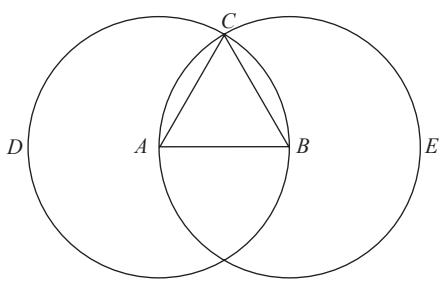
\includegraphics[width=0.42\linewidth]{images/7f061bad1266dd45dcb307a48af1a0707f44763a1fbfbd168a0d78906e1cf15d.jpg}
\caption{Proposition 1 diagram / 命题 1 图}
\end{figure}

\noindent\textbf{English.} Now, since the point $A$ is the centre of the circle $CDB$, $AC$ is equal to $AB$. [Def. 15] Again, since the point $B$ is the centre of the circle $CAE$, $BC$ is equal to $BA$. [Def. 15] But $CA$ was also proved equal to $AB$; therefore each of the straight lines $CA$, $CB$ is equal to $AB$. And things which are equal to the same thing are also equal to one another; [C.N. 1] therefore $CA$ is also equal to $CB$. Therefore the three straight lines $CA$, $AB$, $BC$ are equal to one another. Therefore the triangle $ABC$ is equilateral, and it has been constructed on the given finite straight line $AB$. Being what it was required to do.

\noindent\textbf{中文。} 现在，因为点 $A$ 是圆 $CDB$ 的圆心，所以 $AC$ 等于 $AB$。[定义 15] 又因为点 $B$ 是圆 $CAE$ 的圆心，所以 $BC$ 等于 $BA$。[定义 15] 但已证明 $CA$ 也等于 $AB$；因此直线 $CA$、$CB$ 各自都等于 $AB$。而等于同一事物的事物彼此相等；[共同概念 1] 所以 $CA$ 也等于 $CB$。因此三条直线 $CA$、$AB$、$BC$ 彼此相等。于是三角形 $ABC$ 是等边三角形，并且它已经作在给定有限直线 $AB$ 上。作图完毕。

\subsubsection*{Proposition 2 / 命题 2}

\noindent\textbf{English.} To place at a given point as an extremity a straight line equal to a given straight line.

\noindent\textbf{中文。} 在给定点处，以该点为端点，作一条等于给定直线的直线。

\begin{figure}[htbp]
\centering
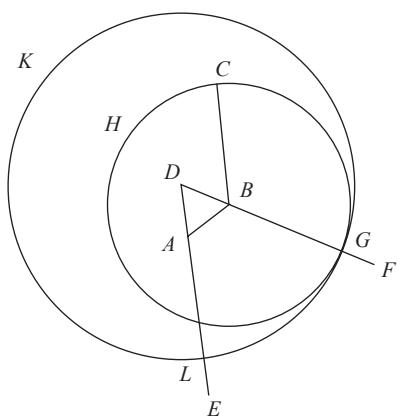
\includegraphics[width=0.44\linewidth]{images/b4e7f322f523fe70254e116490df11c37d34cc0bd8d8545e455ccb1eac3c7c8b.jpg}
\caption{Proposition 2 diagram / 命题 2 图}
\end{figure}

\noindent\textbf{English.} Let $A$ be the given point, and $BC$ the given straight line. Thus it is required to place at the point $A$ as an extremity a straight line equal to the given straight line $BC$. From the point $A$ to the point $B$ let the straight line $AB$ be joined; [Post. 1] and on it let the equilateral triangle $DAB$ be constructed. [I. 1] Let the straight lines $AE$, $BF$ be produced in a straight line with $DA$, $DB$; [Post. 2] with centre $B$ and distance $BC$ let the circle $CGH$ be described; [Post. 3] and again, with centre $D$ and distance $DG$ let the circle $GKL$ be described. [Post. 3]

\noindent\textbf{中文。} 设 $A$ 为给定点，$BC$ 为给定直线。因此要求在点 $A$ 处，以 $A$ 为端点，作一条等于给定直线 $BC$ 的直线。从点 $A$ 到点 $B$ 连接直线 $AB$；[公设 1] 并在其上作等边三角形 $DAB$。[I. 1] 将直线 $AE$、$BF$ 分别沿 $DA$、$DB$ 的方向延长成直线；[公设 2] 以 $B$ 为圆心、$BC$ 为距离作圆 $CGH$；[公设 3] 再以 $D$ 为圆心、$DG$ 为距离作圆 $GKL$。[公设 3]

\noindent\textbf{English.} Then, since the point $B$ is the centre of the circle $CGH$, $BC$ is equal to $BG$. Again, since the point $D$ is the centre of the circle $GKL$, $DL$ is equal to $DG$. And in these $DA$ is equal to $DB$; therefore the remainder $AL$ is equal to the remainder $BG$. [C.N. 3] But $BC$ was also proved equal to $BG$; therefore each of the straight lines $AL$, $BC$ is equal to $BG$. And things which are equal to the same thing are also equal to one another; [C.N. 1] therefore $AL$ is also equal to $BC$. Therefore at the given point $A$ the straight line $AL$ is placed equal to the given straight line $BC$. Being what it was required to do.

\noindent\textbf{中文。} 于是，因为点 $B$ 是圆 $CGH$ 的圆心，所以 $BC$ 等于 $BG$。又因为点 $D$ 是圆 $GKL$ 的圆心，所以 $DL$ 等于 $DG$。而其中 $DA$ 等于 $DB$；因此余下的 $AL$ 等于余下的 $BG$。[共同概念 3] 但已证明 $BC$ 也等于 $BG$；所以直线 $AL$、$BC$ 各自都等于 $BG$。等于同一事物的事物彼此相等；[共同概念 1] 因此 $AL$ 也等于 $BC$。所以在给定点 $A$ 处，已经作出直线 $AL$，使它等于给定直线 $BC$。作图完毕。

\subsubsection*{Proposition 3 / 命题 3}

\noindent\textbf{English.} Given two unequal straight lines, to cut off from the greater a straight line equal to the less.

\noindent\textbf{中文。} 给定两条不相等的直线，从较大者上截取一条等于较小者的直线。

\noindent\textbf{English.} Let $AB$, $C$ be the two given unequal straight lines, and let $AB$ be the greater of them. Thus it is required to cut off from $AB$ the greater a straight line equal to $C$ the less. At the point $A$ let $AD$ be placed equal to the straight line $C$; [I. 2] and with centre $A$ and distance $AD$ let the circle $DEF$ be described. [Post. 3]

\noindent\textbf{中文。} 设 $AB$、$C$ 为给定的两条不相等直线，并设 $AB$ 为其中较大者。因此要求从较大的 $AB$ 上截取一条等于较小的 $C$ 的直线。在点 $A$ 处作 $AD$ 等于直线 $C$；[I. 2] 并以 $A$ 为圆心、$AD$ 为距离作圆 $DEF$。[公设 3]

\begin{figure}[htbp]
\centering
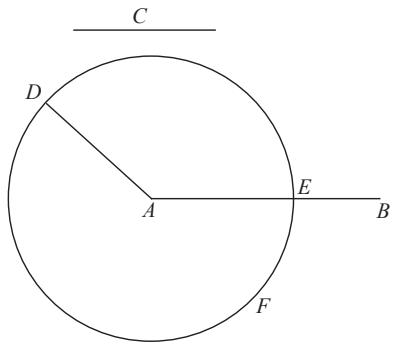
\includegraphics[width=0.42\linewidth]{images/b6842ec6cac3d03b97eeae0e44cf38e34f337eaf8e080ecf2e6add1f7e90b52d.jpg}
\caption{Proposition 3 diagram / 命题 3 图}
\end{figure}

\noindent\textbf{English.} Now, since the point $A$ is the centre of the circle $DEF$, $AE$ is equal to $AD$. [Def. 15] But $C$ is also equal to $AD$. Therefore each of the straight lines $AE$, $C$ is equal to $AD$; so that $AE$ is also equal to $C$. [C.N. 1] Therefore, given the two straight lines $AB$, $C$, from $AB$ the greater, $AE$ has been cut off equal to $C$ the less. Being what it was required to do.

\noindent\textbf{中文。} 现在，因为点 $A$ 是圆 $DEF$ 的圆心，所以 $AE$ 等于 $AD$。[定义 15] 但 $C$ 也等于 $AD$。因此直线 $AE$ 与 $C$ 各自都等于 $AD$；所以 $AE$ 也等于 $C$。[共同概念 1] 因此，给定直线 $AB$、$C$ 时，已从较大的 $AB$ 上截取 $AE$，使其等于较小的 $C$。作图完毕。

\subsubsection*{Proposition 4 / 命题 4}

\noindent\textbf{English.} If two triangles have the two sides equal to two sides respectively, and have the angles contained by the equal straight lines equal, they will also have the base equal to the base, the triangle will be equal to the triangle, and the remaining angles will be equal to the remaining angles respectively, namely those which the equal sides subtend.

\noindent\textbf{中文。} 若两个三角形有两边分别等于两边，且由这些相等直线所夹的角相等，则它们的底也等于底，三角形也等于三角形，其余各角也分别相等，也就是相等边所对的那些角相等。

\noindent\textbf{English.} Let $ABC$, $DEF$ be two triangles having the two sides $AB$, $AC$ equal to the two sides $DE$, $DF$ respectively, namely $AB$ to $DE$ and $AC$ to $DF$, and the angle $BAC$ equal to the angle $EDF$.

\noindent\textbf{中文。} 设 $ABC$、$DEF$ 为两个三角形，其中两边 $AB$、$AC$ 分别等于两边 $DE$、$DF$，即 $AB$ 等于 $DE$、$AC$ 等于 $DF$，并且角 $BAC$ 等于角 $EDF$。

\begin{figure}[htbp]
\centering
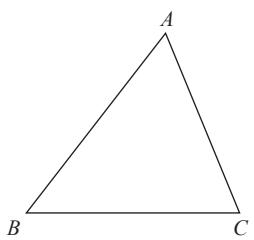
\includegraphics[width=0.28\linewidth]{images/080368f507e9eeb9ca14bad79c3117321aca4e45fc4883ad9766bea1bbf85251.jpg}\quad
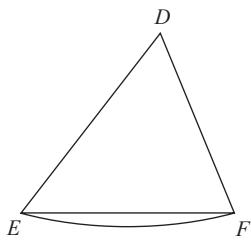
\includegraphics[width=0.28\linewidth]{images/3c3f07b8219daea331169214d575bfc595f88e160f9bab12d7f1619b66c2e404.jpg}
\caption{Proposition 4 diagram / 命题 4 图}
\end{figure}

\noindent\textbf{English.} I say that the base $BC$ is also equal to the base $EF$, the triangle $ABC$ will be equal to the triangle $DEF$, and the remaining angles will be equal to the remaining angles respectively, namely those which the equal sides subtend, that is, the angle $ABC$ to the angle $DEF$, and the angle $ACB$ to the angle $DFE$.

\noindent\textbf{中文。} 我说，底 $BC$ 也等于底 $EF$，三角形 $ABC$ 等于三角形 $DEF$，其余各角也分别相等，即相等边所对的角相等，也就是角 $ABC$ 等于角 $DEF$，角 $ACB$ 等于角 $DFE$。

\noindent\textbf{English.} For, if the triangle $ABC$ be applied to the triangle $DEF$, and if the point $A$ be placed on the point $D$ and the straight line $AB$ on $DE$, then the point $B$ will also coincide with $E$, because $AB$ is equal to $DE$. Again, $AB$ coinciding with $DE$, the straight line $AC$ will also coincide with $DF$, because the angle $BAC$ is equal to the angle $EDF$; hence the point $C$ will also coincide with the point $F$, because $AC$ is again equal to $DF$.

\noindent\textbf{中文。} 因为，如果把三角形 $ABC$ 叠合到三角形 $DEF$ 上，使点 $A$ 放在点 $D$ 上，直线 $AB$ 放在 $DE$ 上，那么点 $B$ 也将与 $E$ 重合，因为 $AB$ 等于 $DE$。再者，当 $AB$ 与 $DE$ 重合时，直线 $AC$ 也将与 $DF$ 重合，因为角 $BAC$ 等于角 $EDF$；于是点 $C$ 也将与点 $F$ 重合，因为 $AC$ 又等于 $DF$。

\noindent\textbf{English.} But $B$ also coincided with $E$; hence the base $BC$ will coincide with the base $EF$ and will be equal to it. [C.N. 4] Thus the whole triangle $ABC$ will coincide with the whole triangle $DEF$ and will be equal to it. And the remaining angles will also coincide with the remaining angles and will be equal to them, the angle $ABC$ to the angle $DEF$, and the angle $ACB$ to the angle $DFE$. Therefore etc. Being what it was required to prove.

\noindent\textbf{中文。} 但 $B$ 也已经与 $E$ 重合；因此底 $BC$ 将与底 $EF$ 重合，并且等于它。[共同概念 4] 于是整个三角形 $ABC$ 将与整个三角形 $DEF$ 重合，并且等于它。其余各角也将与其余各角重合并相等，即角 $ABC$ 等于角 $DEF$，角 $ACB$ 等于角 $DFE$。所以等等。证毕。

\subsubsection*{Proposition 5 / 命题 5}

\noindent\textbf{English.} In isosceles triangles the angles at the base are equal to one another; and, if the equal straight lines be produced further, the angles under the base will be equal to one another.

\noindent\textbf{中文。} 在等腰三角形中，底上的两角彼此相等；并且，如果相等的直线继续延长，则底下的两角也彼此相等。

\noindent\textbf{English.} Let $ABC$ be an isosceles triangle having the side $AB$ equal to the side $AC$; and let the straight lines $BD$, $CE$ be produced further in a straight line with $AB$, $AC$. [Post. 2] I say that the angle $ABC$ is equal to the angle $ACB$, and the angle $CBD$ to the angle $BCE$.

\noindent\textbf{中文。} 设 $ABC$ 为等腰三角形，其中边 $AB$ 等于边 $AC$；并将直线 $BD$、$CE$ 分别沿 $AB$、$AC$ 继续延长成直线。[公设 2] 我说，角 $ABC$ 等于角 $ACB$，且角 $CBD$ 等于角 $BCE$。

\noindent\textbf{English.} Let a point $F$ be taken at random on $BD$; from $AE$ the greater let $AG$ be cut off equal to $AF$ the less; [I. 3] and let the straight lines $FC$, $GB$ be joined. [Post. 1] Then, since $AF$ is equal to $AG$ and $AB$ to $AC$, the two sides $FA$, $AC$ are equal to the two sides $GA$, $AB$, respectively; and they contain a common angle, the angle $FAG$.

\noindent\textbf{中文。} 在 $BD$ 上任取一点 $F$；从较大的 $AE$ 上截取 $AG$，使其等于较小的 $AF$；[I. 3] 并连接直线 $FC$、$GB$。[公设 1] 于是，由于 $AF$ 等于 $AG$，且 $AB$ 等于 $AC$，两边 $FA$、$AC$ 分别等于两边 $GA$、$AB$；并且它们夹着公共角，即角 $FAG$。

\begin{figure}[htbp]
\centering
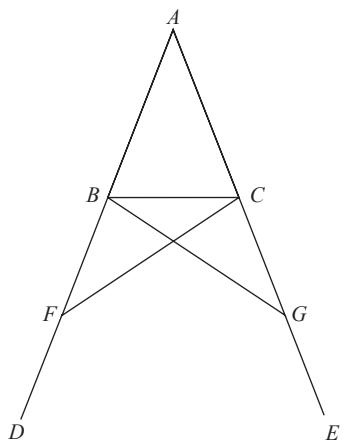
\includegraphics[width=0.42\linewidth]{images/6b61f2fdc0064be390f614c6c8bc31d5431a4c86b8c9c1ecf3f622e794bc177f.jpg}
\caption{Proposition 5 diagram / 命题 5 图}
\end{figure}

\noindent\textbf{English.} Therefore the base $FC$ is equal to the base $GB$, and the triangle $AFC$ is equal to the triangle $AGB$, and the remaining angles will be equal to the remaining angles respectively, namely those which the equal sides subtend, that is, the angle $ACF$ to the angle $ABG$, and the angle $AFC$ to the angle $AGB$. [I. 4]

\noindent\textbf{中文。} 因此底 $FC$ 等于底 $GB$，三角形 $AFC$ 等于三角形 $AGB$，其余各角也分别相等，即相等边所对的角相等，也就是角 $ACF$ 等于角 $ABG$，角 $AFC$ 等于角 $AGB$。[I. 4]

\noindent\textbf{English.} And, since the whole $AF$ is equal to the whole $AG$, and in these $AB$ is equal to $AC$, the remainder $BF$ is equal to the remainder $CG$. But $FC$ was also proved equal to $GB$; therefore the two sides $BF$, $FC$ are equal to the two sides $CG$, $GB$ respectively; and the angle $BFC$ is equal to the angle $CGB$, while the base $BC$ is common to them; therefore the triangle $BFC$ is also equal to the triangle $CGB$, and the remaining angles will be equal to the remaining angles respectively, namely those which the equal sides subtend; therefore the angle $FBC$ is equal to the angle $GCB$, and the angle $BCF$ to the angle $CBG$.

\noindent\textbf{中文。} 又因为整个 $AF$ 等于整个 $AG$，且其中 $AB$ 等于 $AC$，所以余下的 $BF$ 等于余下的 $CG$。但已证明 $FC$ 等于 $GB$；因此两边 $BF$、$FC$ 分别等于两边 $CG$、$GB$；并且角 $BFC$ 等于角 $CGB$，而底 $BC$ 为二者共有；所以三角形 $BFC$ 也等于三角形 $CGB$，其余各角也分别相等，即相等边所对的角相等；因此角 $FBC$ 等于角 $GCB$，角 $BCF$ 等于角 $CBG$。

\noindent\textbf{English.} Accordingly, since the whole angle $ABG$ was proved equal to the angle $ACF$, and in these the angle $CBG$ is equal to the angle $BCF$, the remaining angle $ABC$ is equal to the remaining angle $ACB$; and they are at the base of the triangle $ABC$. But the angle $FBC$ was also proved equal to the angle $GCB$; and they are under the base. Therefore etc. Q.E.D.

\noindent\textbf{中文。} 因此，既然已证明整个角 $ABG$ 等于角 $ACF$，并且其中角 $CBG$ 等于角 $BCF$，则余下的角 $ABC$ 等于余下的角 $ACB$；它们是三角形 $ABC$ 的底角。但也已经证明角 $FBC$ 等于角 $GCB$；它们是底下的角。所以等等。证毕。

\noindent\textbf{English.} [\ldots]

\noindent\textbf{中文。} [原文此处省略]

\subsubsection*{Proposition 7 / 命题 7}

\noindent\textbf{English.} Given two straight lines constructed on a straight line from its extremities and meeting in a point, there cannot be constructed on the same straight line from its extremities, and on the same side of it, two other straight lines meeting in another point and equal to the former two respectively, namely each to that which has the same extremity with it.

\noindent\textbf{中文。} 若从一条直线的两个端点作两条直线并交于一点，则不能在同一条直线的同一侧、仍从其两个端点再作另外两条直线，使它们交于另一点，并且分别等于前两条直线，也就是每一条都等于与它有同一端点的那一条。

\begin{figure}[htbp]
\centering
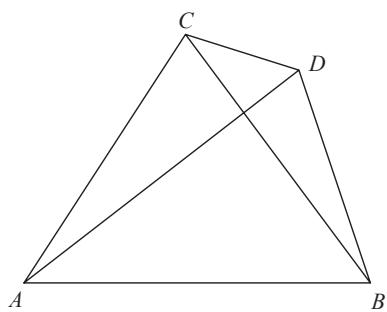
\includegraphics[width=0.42\linewidth]{images/828e9536c5eaa73dcb439a1abef7a7741489914511ed1091710b81aac5f2cffe.jpg}
\caption{Proposition 7 diagram / 命题 7 图}
\end{figure}

\noindent\textbf{English.} For, if possible, given two straight lines $AC$, $CB$ constructed on the straight line $AB$ and meeting at the point $C$, let two other straight lines $AD$, $DB$ be constructed on the same straight line $AB$, on the same side of it, meeting in another point $D$ and equal to the former two respectively, namely each to that which has the same extremity with it, so that $CA$ is equal to $DA$ which has the same extremity $A$ with it, and $CB$ to $DB$ which has the same extremity $B$ with it; and let $CD$ be joined.

\noindent\textbf{中文。} 因为，若可能，给定在直线 $AB$ 上从其端点作出的两条直线 $AC$、$CB$，它们交于点 $C$；设还能在同一条直线 $AB$ 的同一侧作另外两条直线 $AD$、$DB$，它们交于另一点 $D$，并分别等于前两条直线，也就是各自等于与它有同一端点的那一条：$CA$ 等于同以 $A$ 为端点的 $DA$，$CB$ 等于同以 $B$ 为端点的 $DB$；再连接 $CD$。

\noindent\textbf{English.} Then, since $AC$ is equal to $AD$, the angle $ACD$ is also equal to the angle $ADC$. [I. 5] Therefore the angle $ADC$ is greater than the angle $DCB$; therefore the angle $CDB$ is much greater than the angle $DCB$. Again, since $CB$ is equal to $DB$, the angle $CDB$ is also equal to the angle $DCB$. But it was also proved much greater than it, which is impossible. Therefore etc. Q.E.D.

\noindent\textbf{中文。} 于是，由于 $AC$ 等于 $AD$，角 $ACD$ 也等于角 $ADC$。[I. 5] 因此角 $ADC$ 大于角 $DCB$；所以角 $CDB$ 更大于角 $DCB$。又由于 $CB$ 等于 $DB$，角 $CDB$ 也等于角 $DCB$。但又已证明它远大于后者，这是不可能的。所以等等。证毕。

\subsubsection*{Proposition 8 / 命题 8}

\noindent\textbf{English.} If two triangles have the two sides equal to two sides respectively, and have also the base equal to the base, they will also have the angles equal which are contained by the equal straight lines.

\noindent\textbf{中文。} 若两个三角形有两边分别等于两边，并且底也等于底，则由这些相等直线所夹的角也相等。

\noindent\textbf{English.} Let $ABC$, $DEF$ be two triangles having the two sides $AB$, $AC$ equal to the two sides $DE$, $DF$ respectively, namely $AB$ to $DE$, and $AC$ to $DF$; and let them have the base $BC$ equal to the base $EF$. I say that the angle $BAC$ is also equal to the angle $EDF$.

\noindent\textbf{中文。} 设 $ABC$、$DEF$ 为两个三角形，其中两边 $AB$、$AC$ 分别等于两边 $DE$、$DF$，即 $AB$ 等于 $DE$，$AC$ 等于 $DF$；并且它们的底 $BC$ 等于底 $EF$。我说，角 $BAC$ 也等于角 $EDF$。

\noindent\textbf{English.} For, if the triangle $ABC$ be applied to the triangle $DEF$, and if the point $B$ be placed on the point $E$ and the straight line $BC$ on $EF$, the point $C$ will also coincide with $F$, because $BC$ is equal to $EF$.

\noindent\textbf{中文。} 因为，如果把三角形 $ABC$ 叠合到三角形 $DEF$ 上，使点 $B$ 放在点 $E$ 上，并使直线 $BC$ 放在 $EF$ 上，那么点 $C$ 也将与 $F$ 重合，因为 $BC$ 等于 $EF$。

\begin{figure}[htbp]
\centering
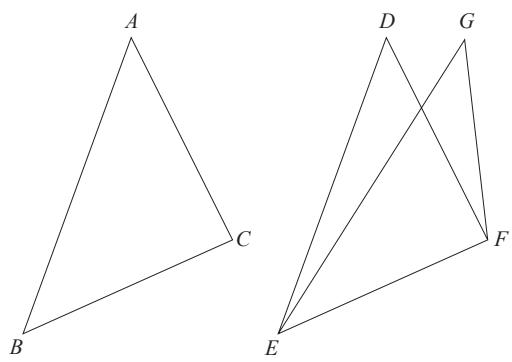
\includegraphics[width=0.42\linewidth]{images/cc70ef0f787dd782c274c6403b90172997502bd074a5e5a5febde01f717b00f6.jpg}
\caption{Proposition 8 diagram / 命题 8 图}
\end{figure}

\noindent\textbf{English.} Then, $BC$ coinciding with $EF$, $BA$, $AC$ will also coincide with $ED$, $DF$; for, if the base $BC$ coincides with the base $EF$, and the sides $BA$, $AC$ do not coincide with $ED$, $DF$ but fall beside them as $EG$, $GF$, then, given two straight lines constructed on a straight line from its extremities and meeting in a point, there will have been constructed on the same straight line from its extremities, and on the same side of it, two other straight lines meeting in another point and equal to the former two respectively, namely each to that which has the same extremity with it. But they cannot be so constructed. [I. 7]

\noindent\textbf{中文。} 然后，当 $BC$ 与 $EF$ 重合时，$BA$、$AC$ 也将与 $ED$、$DF$ 重合；因为，如果底 $BC$ 与底 $EF$ 重合，而边 $BA$、$AC$ 不与 $ED$、$DF$ 重合，却落在旁边成为 $EG$、$GF$，那么就会出现这样的情况：从一条直线的两个端点作两条直线并交于一点之后，又在同一条直线的同一侧、从其两个端点作出另外两条直线，交于另一点，并分别等于前两条直线，也就是每条都等于与它有同一端点的那条。但这样的作图不可能。[I. 7]

\noindent\textbf{English.} Therefore it is not possible that, if the base $BC$ be applied to the base $EF$, the sides $BA$, $AC$ should not coincide with $ED$, $DF$; they will therefore coincide, so that the angle $BAC$ will also coincide with the angle $EDF$, and will be equal to it. If therefore etc. Q.E.D.

\noindent\textbf{中文。} 因此，如果底 $BC$ 叠合到底 $EF$ 上，边 $BA$、$AC$ 不与 $ED$、$DF$ 重合是不可能的；所以它们将重合，从而角 $BAC$ 也将与角 $EDF$ 重合，并且等于它。所以等等。证毕。

\subsubsection*{Proposition 9 / 命题 9}

\noindent\textbf{English.} To bisect a given rectilineal angle.

\noindent\textbf{中文。} 平分给定直线角。

\begin{figure}[htbp]
\centering
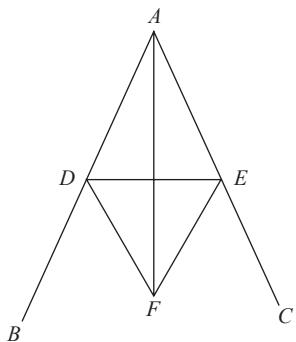
\includegraphics[width=0.42\linewidth]{images/c15463dc3ef129c034e9bda5835bcfe11a3503c0ed6d14430e248712df29c268.jpg}
\caption{Proposition 9 diagram / 命题 9 图}
\end{figure}

\noindent\textbf{English.} Let the angle $BAC$ be the given rectilineal angle. Thus it is required to bisect it. Let a point $D$ be taken at random on $AB$; let $AE$ be cut off from $AC$ equal to $AD$; [I. 3] let $DE$ be joined, and on $DE$ let the equilateral triangle $DEF$ be constructed; let $AF$ be joined. I say that the angle $BAC$ has been bisected by the straight line $AF$.

\noindent\textbf{中文。} 设角 $BAC$ 为给定直线角。因此要求平分它。在 $AB$ 上任取一点 $D$；从 $AC$ 上截取 $AE$，使其等于 $AD$；[I. 3] 连接 $DE$，并在 $DE$ 上作等边三角形 $DEF$；连接 $AF$。我说，角 $BAC$ 已被直线 $AF$ 平分，$AF$ 即为角平分线。

\noindent\textbf{English.} For, since $AD$ is equal to $AE$, and $AF$ is common, the two sides $DA$, $AF$ are equal to the two sides $EA$, $AF$ respectively. And the base $DF$ is equal to the base $EF$; therefore the angle $DAF$ is equal to the angle $EAF$. [I. 8] Therefore the given rectilineal angle $BAC$ has been bisected by the straight line $AF$. Q.E.F.

\noindent\textbf{中文。} 因为 $AD$ 等于 $AE$，且 $AF$ 为公共边，所以两边 $DA$、$AF$ 分别等于两边 $EA$、$AF$。又底 $DF$ 等于底 $EF$；因此角 $DAF$ 等于角 $EAF$。[I. 8] 所以给定直线角 $BAC$ 已由直线 $AF$ 平分。作图完毕。

\subsubsection*{Proposition 10 / 命题 10}

\noindent\textbf{English.} To bisect a given finite straight line.

\noindent\textbf{中文。} 平分给定有限直线。

\begin{figure}[htbp]
\centering
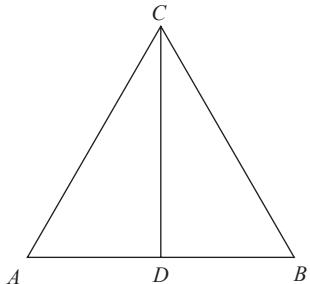
\includegraphics[width=0.42\linewidth]{images/344770768dd08da63064ff9c20f95022735918a2610550ba8f0f158d481aafb2.jpg}
\caption{Proposition 10 diagram / 命题 10 图}
\end{figure}

\noindent\textbf{English.} Let $AB$ be the given finite straight line. Thus it is required to bisect the finite straight line $AB$. Let the equilateral triangle $ABC$ be constructed on it, [I. 1] and let the angle $ACB$ be bisected by the straight line $CD$; [I. 9] I say that the straight line $AB$ has been bisected at the point $D$.

\noindent\textbf{中文。} 设 $AB$ 为给定有限直线。因此要求平分有限直线 $AB$。在其上作等边三角形 $ABC$，[I. 1] 并由直线 $CD$ 平分角 $ACB$；[I. 9] 我说，直线 $AB$ 已在点 $D$ 处被平分。

\noindent\textbf{English.} For, since $AC$ is equal to $CB$, and $CD$ is common, the two sides $AC$, $CD$ are equal to the two sides $BC$, $CD$ respectively; and the angle $ACD$ is equal to the angle $BCD$; [I. 4] therefore the base $AD$ is equal to the base $BD$. Therefore the given finite straight line $AB$ has been bisected at $D$. Q.E.F.

\noindent\textbf{中文。} 因为 $AC$ 等于 $CB$，且 $CD$ 为公共边，所以两边 $AC$、$CD$ 分别等于两边 $BC$、$CD$；并且角 $ACD$ 等于角 $BCD$；[I. 4] 因此底 $AD$ 等于底 $BD$。所以给定有限直线 $AB$ 已在 $D$ 处被平分。作图完毕。

\subsubsection*{Proposition 11 / 命题 11}

\noindent\textbf{English.} To draw a straight line at right angles to a given straight line from a given point on it.

\noindent\textbf{中文。} 从给定直线上的给定点，作一条与该给定直线成直角的直线。

\noindent\textbf{English.} Let $AB$ be the given straight line, and $C$ the given point on it. Thus it is required to draw from the point $C$ a straight line at right angles to the straight line $AB$. Let a point $D$ be taken at random on $AC$; let $CE$ be made equal to $CD$; [I. 3] on $DE$ let the equilateral triangle $FDE$ be constructed, [I. 1] and let $FC$ be joined.

\noindent\textbf{中文。} 设 $AB$ 为给定直线，$C$ 为其上的给定点。因此要求从点 $C$ 作一条与直线 $AB$ 成直角的直线。在 $AC$ 上任取一点 $D$；令 $CE$ 等于 $CD$；[I. 3] 在 $DE$ 上作等边三角形 $FDE$，[I. 1] 并连接 $FC$。

\begin{figure}[htbp]
\centering
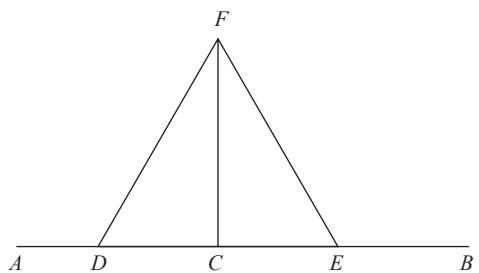
\includegraphics[width=0.42\linewidth]{images/b9a58f36da06f5759bed049e2bb3826aa61e46c8c908e86e50ce69ade03b3e96.jpg}
\caption{Proposition 11 diagram / 命题 11 图}
\end{figure}

\noindent\textbf{English.} I say that the straight line $FC$ has been drawn at right angles to the given straight line $AB$ from $C$, the given point on it. For, since $DC$ is equal to $CE$, and $CF$ is common, the two sides $DC$, $CF$ are equal to the two sides $EC$, $CF$ respectively; and the base $DF$ is equal to the base $FE$; therefore the angle $DCF$ is equal to the angle $ECF$; [I. 8] and they are adjacent angles.

\noindent\textbf{中文。} 我说，已经从给定直线 $AB$ 上的给定点 $C$ 作出与 $AB$ 成直角的直线 $FC$。因为 $DC$ 等于 $CE$，且 $CF$ 为公共边，所以两边 $DC$、$CF$ 分别等于两边 $EC$、$CF$；并且底 $DF$ 等于底 $FE$；因此角 $DCF$ 等于角 $ECF$；[I. 8] 而它们是相邻角。

\noindent\textbf{English.} But, when a straight line set up on a straight line makes the adjacent angles equal to one another, each of the equal angles is right; [Def. 10] therefore each of the angles $DCF$, $FCE$ is right. Therefore the straight line $CF$ has been drawn at right angles to the given straight line $AB$ from the given point $C$ on it. Q.E.F.

\noindent\textbf{中文。} 但当一条直线立在另一条直线上并使相邻角彼此相等时，每一个相等的角都是直角；[定义 10] 所以角 $DCF$、$FCE$ 都是直角。因此，已经从给定直线 $AB$ 上的给定点 $C$ 作出与之成直角的直线 $CF$，即一条垂线。作图完毕。

\noindent\textbf{English.} [\ldots]

\noindent\textbf{中文。} [原文此处省略]

\subsubsection*{Proposition 13 / 命题 13}

\noindent\textbf{English.} If a straight line set up on a straight line make angles, it will make either two right angles or angles equal to two right angles.

\noindent\textbf{中文。} 若一条直线立在另一条直线上而成角，则它所成的要么是两个直角，要么是和等于两个直角的角。

\begin{figure}[htbp]
\centering
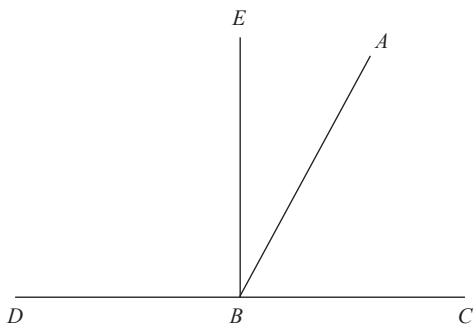
\includegraphics[width=0.42\linewidth]{images/71267a012817a97b765d3c633d03d379115716b87ef23ca8d5302d010a8a8c11.jpg}
\caption{Proposition 13 diagram / 命题 13 图}
\end{figure}

\noindent\textbf{English.} For let any straight line $AB$ set up on the straight line $CD$ make the angles $CBA$, $ABD$; I say that the angles $CBA$, $ABD$ are either two right angles or equal to two right angles. Now, if the angle $CBA$ is equal to the angle $ABD$, they are two right angles. [Def. 10]

\noindent\textbf{中文。} 设任一直线 $AB$ 立在直线 $CD$ 上，形成角 $CBA$、$ABD$；我说，角 $CBA$、$ABD$ 要么是两个直角，要么其和等于两个直角。现在，如果角 $CBA$ 等于角 $ABD$，它们就是两个直角。[定义 10]

\noindent\textbf{English.} But, if not, let $BE$ be drawn from the point $B$ at right angles to $CD$; [I. 11] therefore the angles $CBE$, $EBD$ are two right angles. Then, since the angle $CBE$ is equal to the two angles $CBA$, $ABE$, let the angle $EBD$ be added to each; therefore the angles $CBE$, $EBD$ are equal to the three angles $CBA$, $ABE$, $EBD$. [C.N. 2] Again, since the angle $DBA$ is equal to the two angles $DBE$, $EBA$, let the angle $ABC$ be added to each; therefore the angles $DBA$, $ABC$ are equal to the three angles $DBE$, $EBA$, $ABC$. [C.N. 2]

\noindent\textbf{中文。} 若不相等，则从点 $B$ 作 $BE$ 垂直于 $CD$；[I. 11] 因此角 $CBE$、$EBD$ 是两个直角。于是，由于角 $CBE$ 等于两个角 $CBA$、$ABE$ 之和，把角 $EBD$ 分别加到两边；所以角 $CBE$、$EBD$ 之和等于三个角 $CBA$、$ABE$、$EBD$ 之和。[共同概念 2] 又由于角 $DBA$ 等于两个角 $DBE$、$EBA$ 之和，把角 $ABC$ 分别加到两边；所以角 $DBA$、$ABC$ 之和等于三个角 $DBE$、$EBA$、$ABC$ 之和。[共同概念 2]

\noindent\textbf{English.} But the angles $CBE$, $EBD$ were also proved equal to the same three angles; and things which are equal to the same thing are also equal to one another; [C.N. 1] therefore the angles $CBE$, $EBD$ are also equal to the angles $DBA$, $ABC$. But the angles $CBE$, $EBD$ are two right angles; therefore the angles $DBA$, $ABC$ are also equal to two right angles. Therefore etc. Q.E.D.

\noindent\textbf{中文。} 但角 $CBE$、$EBD$ 也已证明等于同样的三个角；而等于同一事物的事物彼此相等；[共同概念 1] 因此角 $CBE$、$EBD$ 也等于角 $DBA$、$ABC$。但角 $CBE$、$EBD$ 是两个直角；所以角 $DBA$、$ABC$ 之和也等于两个直角。所以等等。证毕。

\noindent\textbf{English.} [\ldots]

\noindent\textbf{中文。} [原文此处省略]

\subsubsection*{Proposition 15 / 命题 15}

\noindent\textbf{English.} If two straight lines cut one another, they make the vertical angles equal to one another.

\noindent\textbf{中文。} 若两条直线相交，则它们所成的对顶角彼此相等。

\noindent\textbf{English.} For let the straight lines $AB$, $CD$ cut one another at the point $E$; I say that the angle $AEC$ is equal to the angle $DEB$, and the angle $CEB$ to the angle $AED$.

\noindent\textbf{中文。} 设直线 $AB$、$CD$ 相交于点 $E$；我说，角 $AEC$ 等于角 $DEB$，角 $CEB$ 等于角 $AED$。

\begin{figure}[htbp]
\centering
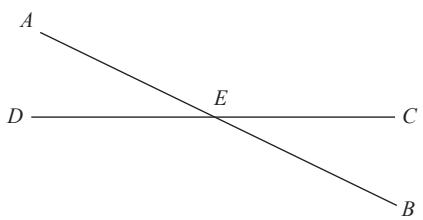
\includegraphics[width=0.42\linewidth]{images/6246ab53667b2e8dc6015ec40cae51efb7530a8d663f20e0861ba3249b47d47c.jpg}
\caption{Proposition 15 diagram / 命题 15 图}
\end{figure}

\noindent\textbf{English.} For, since the straight line $AE$ stands on the straight line $CD$, making the angles $CEA$, $AED$, the angles $CEA$, $AED$ are equal to two right angles. [I. 13] Again, since the straight line $DE$ stands on the straight line $AB$, making the angles $AED$, $DEB$, the angles $AED$, $DEB$ are equal to two right angles. [I. 13]

\noindent\textbf{中文。} 因为直线 $AE$ 立在直线 $CD$ 上，形成角 $CEA$、$AED$，所以角 $CEA$、$AED$ 之和等于两个直角。[I. 13] 又由于直线 $DE$ 立在直线 $AB$ 上，形成角 $AED$、$DEB$，所以角 $AED$、$DEB$ 之和等于两个直角。[I. 13]

\noindent\textbf{English.} But the angles $CEA$, $AED$ were also proved equal to two right angles; therefore the angles $CEA$, $AED$ are equal to the angles $AED$, $DEB$. [Post. 4 and C.N. 1] Let the angle $AED$ be subtracted from each; therefore the remaining angle $CEA$ is equal to the remaining angle $BED$. [C.N. 3] Similarly it can be proved that the angles $CEB$, $DEA$ are also equal. Therefore etc. Q.E.D.

\noindent\textbf{中文。} 但角 $CEA$、$AED$ 也已证明等于两个直角；因此角 $CEA$、$AED$ 之和等于角 $AED$、$DEB$ 之和。[公设 4 与共同概念 1] 从两边减去角 $AED$；于是余下的角 $CEA$ 等于余下的角 $BED$。[共同概念 3] 同理可证，角 $CEB$、$DEA$ 也相等。所以等等。证毕。

\noindent\textbf{English.} [\ldots]

\noindent\textbf{中文。} [原文此处省略]

\subsubsection*{Proposition 16 / 命题 16}

\noindent\textbf{English.} In any triangle, if one of the sides be produced, the exterior angle is greater than either of the interior and opposite angles.

\noindent\textbf{中文。} 在任意三角形中，若延长一边，则外角大于任一不相邻内角。

\noindent\textbf{English.} Let $ABC$ be a triangle, and let one side of it $BC$ be produced to $D$; I say that the exterior angle $ACD$ is greater than either of the interior and opposite angles $CBA$, $BAC$. Let $AC$ be bisected at $E$, [I. 10] and let $BE$ be joined and produced in a straight line to $F$.

\noindent\textbf{中文。} 设 $ABC$ 为三角形，并将其一边 $BC$ 延长到 $D$；我说，外角 $ACD$ 大于任一内对角 $CBA$、$BAC$。令 $AC$ 在 $E$ 处被平分，[I. 10] 并连接 $BE$，再沿直线延长到 $F$。

\begin{figure}[htbp]
\centering
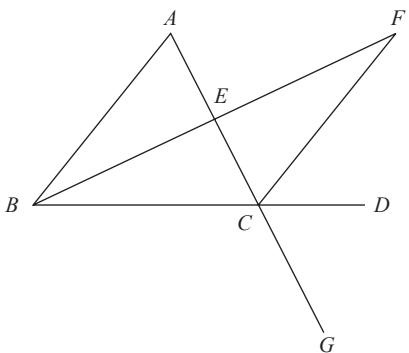
\includegraphics[width=0.42\linewidth]{images/6b4a6abdc4714f5762c7b8e3be81141be8ef74db03fbf56119ba30fb31e25698.jpg}
\caption{Proposition 16 diagram / 命题 16 图}
\end{figure}

\noindent\textbf{English.} Let $EF$ be made equal to $BE$, [I. 3] let $FC$ be joined, [Post. 1] and let $AC$ be drawn through to $G$. [Post. 2] Then, since $AE$ is equal to $EC$, and $BE$ to $EF$, the two sides $AE$, $EB$ are equal to the two sides $CE$, $EF$ respectively; and the angle $AEB$ is equal to the angle $FEC$, for they are vertical angles. [I. 15] Therefore the base $AB$ is equal to the base $FC$, and the triangle $ABE$ is equal to the triangle $CFE$, and the remaining angles are equal to the remaining angles respectively, namely those which the equal sides subtend; [I. 4] therefore the angle $BAE$ is equal to the angle $ECF$.

\noindent\textbf{中文。} 令 $EF$ 等于 $BE$，[I. 3] 连接 $FC$，[公设 1] 并将 $AC$ 延长到 $G$。[公设 2] 于是，由于 $AE$ 等于 $EC$，且 $BE$ 等于 $EF$，两边 $AE$、$EB$ 分别等于两边 $CE$、$EF$；而角 $AEB$ 等于角 $FEC$，因为它们是对顶角。[I. 15] 因此底 $AB$ 等于底 $FC$，三角形 $ABE$ 等于三角形 $CFE$，其余各角也分别相等，即相等边所对的角相等；[I. 4] 所以角 $BAE$ 等于角 $ECF$。

\noindent\textbf{English.} But the angle $ECD$ is greater than the angle $ECF$; [C.N. 5] therefore the angle $ACD$ is greater than the angle $BAE$. Similarly also, if $BC$ be bisected, the angle $BCG$, that is, the angle $ACD$, [I. 15] can be proved greater than the angle $ABC$ as well. Therefore etc. Q.E.D.

\noindent\textbf{中文。} 但角 $ECD$ 大于角 $ECF$；[共同概念 5] 因此角 $ACD$ 大于角 $BAE$。同样，若平分 $BC$，也可证明角 $BCG$，也就是角 $ACD$，[I. 15] 大于角 $ABC$。所以等等。证毕。

\noindent\textbf{English.} [\ldots]

\noindent\textbf{中文。} [原文此处省略]

\subsubsection*{Proposition 18 / 命题 18}

\noindent\textbf{English.} In any triangle the greater side subtends the greater angle.

\noindent\textbf{中文。} 在任意三角形中，较大的边对较大的角。

\begin{figure}[htbp]
\centering
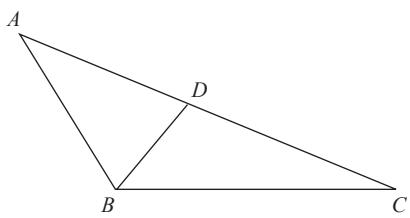
\includegraphics[width=0.42\linewidth]{images/d9da22780dfcf229f4edbdb0297898dcad5788013f8abf1785e53626f11eaccb.jpg}
\caption{Proposition 18 diagram / 命题 18 图}
\end{figure}

\noindent\textbf{English.} For let $ABC$ be a triangle having the side $AC$ greater than $AB$; I say that the angle $ABC$ is also greater than the angle $BCA$. For, since $AC$ is greater than $AB$, let $AD$ be made equal to $AB$; [I. 3] and let $BD$ be joined. Then, since the angle $ADB$ is an exterior angle of the triangle $BCD$, it is greater than the interior and opposite angle $DCB$. But the angle $ADB$ is equal to the angle $ABD$, since the side $AB$ is equal to $AD$; [I. 5] therefore the angle $ABD$ is also greater than the angle $ACB$; therefore the angle $ABC$ is much greater than the angle $ACB$. Therefore etc. Q.E.D.

\noindent\textbf{中文。} 设 $ABC$ 为三角形，且边 $AC$ 大于 $AB$；我说，角 $ABC$ 也大于角 $BCA$。因为 $AC$ 大于 $AB$，令 $AD$ 等于 $AB$；[I. 3] 并连接 $BD$。于是，由于角 $ADB$ 是三角形 $BCD$ 的外角，它大于内对角 $DCB$。但角 $ADB$ 等于角 $ABD$，因为边 $AB$ 等于 $AD$；[I. 5] 因此角 $ABD$ 也大于角 $ACB$；所以角 $ABC$ 更大于角 $ACB$。所以等等。证毕。

\subsubsection*{Proposition 19 / 命题 19}

\noindent\textbf{English.} In any triangle the greater angle is subtended by the greater side.

\noindent\textbf{中文。} 在任意三角形中，较大的角由较大的边所对。

\noindent\textbf{English.} Let $ABC$ be a triangle having the angle $ABC$ greater than the angle $BCA$; I say that the side $AC$ is also greater than the side $AB$. For, if not, $AC$ is either equal to $AB$ or less. Now $AC$ is not equal to $AB$; for then the angle $ABC$ would also have been equal to the angle $ACB$; [I. 5] but it is not.

\noindent\textbf{中文。} 设 $ABC$ 为三角形，且角 $ABC$ 大于角 $BCA$；我说，边 $AC$ 也大于边 $AB$。因为若不然，$AC$ 要么等于 $AB$，要么小于 $AB$。现在 $AC$ 不等于 $AB$；否则角 $ABC$ 也会等于角 $ACB$；[I. 5] 但它并不相等。

\begin{figure}[htbp]
\centering
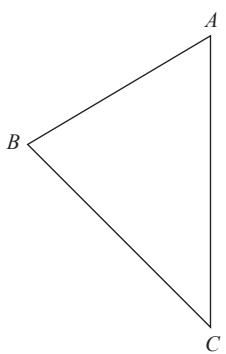
\includegraphics[width=0.42\linewidth]{images/302a6c393eebc8820de0cfd0af310f1bc81e9a0762c586c845292d64ed567da0.jpg}
\caption{Proposition 19 diagram / 命题 19 图}
\end{figure}

\noindent\textbf{English.} Therefore $AC$ is not equal to $AB$. Neither is $AC$ less than $AB$, for then the angle $ABC$ would also have been less than the angle $ACB$; [I. 18] but it is not; therefore $AC$ is not less than $AB$. And it was proved that it is not equal either. Therefore $AC$ is greater than $AB$. Therefore etc. Q.E.D.

\noindent\textbf{中文。} 因此 $AC$ 不等于 $AB$。$AC$ 也不小于 $AB$，因为若小于，则角 $ABC$ 也会小于角 $ACB$；[I. 18] 但事实并非如此；因此 $AC$ 不小于 $AB$。又已证明它也不相等。所以 $AC$ 大于 $AB$。所以等等。证毕。

\subsubsection*{Proposition 20 / 命题 20}

\noindent\textbf{English.} In any triangle two sides taken together in any manner are greater than the remaining one.

\noindent\textbf{中文。} 在任意三角形中，任取两边之和都大于余下的一边。

\noindent\textbf{English.} For let $ABC$ be a triangle; I say that in the triangle $ABC$ two sides taken together in any manner are greater than the remaining one, namely $BA$, $AC$ greater than $BC$, $AB$, $BC$ greater than $AC$, and $BC$, $CA$ greater than $AB$.

\noindent\textbf{中文。} 设 $ABC$ 为三角形；我说，在三角形 $ABC$ 中，任取两边之和都大于余下的一边，即 $BA$、$AC$ 之和大于 $BC$，$AB$、$BC$ 之和大于 $AC$，$BC$、$CA$ 之和大于 $AB$。

\begin{figure}[htbp]
\centering
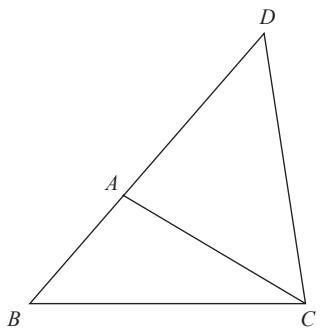
\includegraphics[width=0.42\linewidth]{images/4f02fa1bc68d5bb688d94c409625e29512d0f27b81961c35b4b9b5890f24a90d.jpg}
\caption{Proposition 20 diagram / 命题 20 图}
\end{figure}

\noindent\textbf{English.} For let $BA$ be drawn through to the point $D$, let $DA$ be made equal to $CA$, and let $DC$ be joined. Then, since $DA$ is equal to $AC$, the angle $ADC$ is also equal to the angle $ACD$; [I. 5] therefore the angle $BCD$ is greater than the angle $ADC$. [C.N. 5]

\noindent\textbf{中文。} 将 $BA$ 延长到点 $D$，令 $DA$ 等于 $CA$，并连接 $DC$。于是，由于 $DA$ 等于 $AC$，角 $ADC$ 也等于角 $ACD$；[I. 5] 因此角 $BCD$ 大于角 $ADC$。[共同概念 5]

\noindent\textbf{English.} And, since $DCB$ is a triangle having the angle $BCD$ greater than the angle $BDC$, and the greater angle is subtended by the greater side, [I. 19] therefore $DB$ is greater than $BC$. But $DA$ is equal to $AC$; therefore $BA$, $AC$ are greater than $BC$. Similarly we can prove that $AB$, $BC$ are also greater than $CA$, and $BC$, $CA$ than $AB$. Therefore etc. Q.E.D.

\noindent\textbf{中文。} 又由于 $DCB$ 是一个三角形，其中角 $BCD$ 大于角 $BDC$，而较大的角由较大的边所对，[I. 19] 所以 $DB$ 大于 $BC$。但 $DA$ 等于 $AC$；因此 $BA$、$AC$ 之和大于 $BC$。同理可证，$AB$、$BC$ 之和也大于 $CA$，$BC$、$CA$ 之和大于 $AB$。所以等等。证毕。
